\documentclass[]{scrartcl}
% Лицензия
% Apache License Version 2.0, January 2004
% http://www.apache.org/licenses/
% Copyright [2020] [Kirill A. Murashev]
% Licensed under the Apache License, Version 2.0 (the "License"); you may not use this file except in compliance with the License. You may obtain a copy of the License at
% http://www.apache.org/licenses/LICENSE-2.0
% Unless required by applicable law or agreed to in writing, software
% distributed under the License is distributed on an "AS IS" BASIS,
% WITHOUT WARRANTIES OR CONDITIONS OF ANY KIND, either express or implied.
% See the License for the specific language governing permissions and limitations under the License.


%%% Работа с русским языком
\usepackage{cmap}					% поиск в PDF
\usepackage{mathtext} 				% русские буквы в формулах
\usepackage{fontspec}
\defaultfontfeatures{Renderer=Basic,Ligatures={TeX}}
\setmainfont{CMU Serif}
\setsansfont{CMU Sans Serif}
\setmonofont{CMU Typewriter Text}
\usepackage[english,russian]{babel}
%\usepackage[T1,T2A]{fontenc}			% кодировка
%\usepackage[lutf8]{luainputenc}			% кодировка исходного текста
%\usepackage[english,russian]{babel}	% локализация и переносы
\usepackage{indentfirst}            % красная строка
\usepackage{misccorr}               % доработки для babel
\frenchspacing                      % французский стиль пробелов

%\usepackage{beton} %изменение шрифта для тёмной цветовой схемы
%\usepackage{concrete}
%%% Дополнительная работа с математикой
\usepackage{amsmath,amsfonts,amssymb,amsthm,mathtools} % AMS
\usepackage{icomma} % "Умная" запятая: $0,2$ --- число, $0, 2$ --- перечисление

%% Номера формул
%\mathtoolsset{showonlyrefs=true} % Показывать номера только у тех формул, на которые есть \eqref{} в тексте.
%\usepackage{leqno} % Нумерация формул слева

%% Перенос знаков в формулах (по Львовскому)
\newcommand*{\hm}[1]{#1\nobreak\discretionary{}
	{\hbox{$\mathsurround=0pt #1$}}{}}

%%% Работа с картинками
\usepackage{graphicx}  % Для вставки рисунков
\graphicspath{{Images/}}  % папки с картинками
\setlength\fboxsep{3pt} % Отступ рамки \fbox{} от рисунка
\setlength\fboxrule{1pt} % Толщина линий рамки \fbox{}
\usepackage{wrapfig} % Обтекание рисунков текстом

%%% Работа с таблицами
\usepackage{array, tabularx, tabulary, booktabs, xtab} % Дополнительная работа с таблицами
\usepackage{longtable}  % Длинные таблицы
\usepackage{multirow} % Слияние строк в таблице

%%% Теоремы
\theoremstyle{plain} % Это стиль по умолчанию, его можно не переопределять.
\newtheorem{theorem}{Теорема}[section]
\newtheorem{proposition}[theorem]{Утверждение}

\theoremstyle{definition} % "Определение"
\newtheorem{corollary}{Следствие}[theorem]
\newtheorem{problem}{Задача}[section]

\theoremstyle{remark} % "Примечание"
\newtheorem*{nonum}{Решение}

%%% Программирование
\usepackage{etoolbox} % логические операторы

\usepackage{lastpage} % Узнать, сколько всего страниц в документе.

\usepackage{keyval}

\usepackage{totcount} % Узнать, сколько всего объектов в документе.

%\usepackage{xcolor-solarized}

%%% Страница
%\usepackage{extsizes} % Возможность сделать 14-й шрифт
%\usepackage{geometry} % Простой способ задавать поля
%	\geometry{top=25mm}
%	\geometry{bottom=35mm}
%	\geometry{left=35mm}
%	\geometry{right=20mm}
%

%\usepackage{fancyhdr} % Колонтитулы

%	\pagestyle{fancy}
%\renewcommand{\headrulewidth}{0pt}  % Толщина линейки, отчеркивающей верхний колонтитул
%\fancyhf{}
%\lhead{Часть \thepart}
%\chead{Глава \thechapter}
%\rhead{Раздел \thesection}
%\lfoot{version 0.251}
%\cfoot{\today} % По умолчанию здесь номер страницы
%\rfoot{\thepage/\ref{LastPage}}
%\pagestyle{fancy}

%\usepackage{setspace} % Интерлиньяж
%\onehalfspacing % Интерлиньяж 1.5
%\doublespacing % Интерлиньяж 2
%\singlespacing % Интерлиньяж 1

\usepackage{soul} % Модификаторы начертания

\usepackage[usenames,dvipsnames,svgnames,table,rgb]{xcolor} % Подключение пакета для задания цвета

%\definecolor{Backcolor}{HTML}{042029} % Задание цвета для фона
%\definecolor{Textcolor}{HTML}{819090} % Задание цвета для текста
%\pagecolor{Backcolor}                 % Подключение тёмной
%\color{Textcolor}                     % темы

\usepackage{csquotes} % Ещё инструменты для ссылок

\usepackage[backend=biber,bibencoding=utf8,sorting=ynt,maxcitenames=5,sortupper=true,date=iso]{biblatex} % подключение пакета для работы с автоматизированной библиографией

%\usepackage[style=authoryear,maxcitenames=2,backend=biber,sorting=nty]{biblatex}

%\renewcommand\bibname{Источники информации} % Переопределение названия для библиографии

\usepackage{multicol} % Несколько колонок

\usepackage{microtype}              %<-- added for better inter word spacing

\usepackage{tabularx}

\usepackage{tikz} % Работа с графикой
\usepackage{pgfplots}
\usepackage{pgfplotstable}

\usepackage{eqlist}

\usepackage{desclist} % Дополнительное окружение для списка Глоссария

\usepackage{lineno} % Нумерация строк

\setcounter{tocdepth}{8} % Глубина оглавления

% подавление висячих строк
\clubpenalty=400 % Разрешение = 300, абсолютный запрет = 10000
\widowpenalty=400 % Увеличиваем эти числа до тех пор, пока не начнёт увеличиваться количество страниц.

% Выбор между разрежением и переполнением
\tolerance=500 % max=10000, default=200

\looseness=-1 % иногда можно удлинять страницу на одну строку.

\hfuzz=2.5pt % иногда можно вылезти за край строки на 2.5 pt.

\usepackage{calc} % Вычисления

\usepackage{scrlayer-scrpage} % Стиль страницы

\usepackage{lineno} % нумерация строк

%\pagestyle{scrpage}

%\usepackage{concrete}

\usepackage{booktabs}

\usepackage[owncaptions]{vhistory} % Log of versions

\usepackage{progressbar} % Формирование линейки, показывающей прогресс в работе

\usepackage{epigraph} % работа с эпиграфами

\usepackage {listings}
\lstloadlanguages{[Latex]Tex, bash, R, Python, SQL}
\lstset{extendedchars=true , % включаем не латиницу
frame=tb, % рамка сверху и снизу
commentstyle=\itshape , % шрифт для комментариев
stringstyle =\ttfamily % шрифт для строк
%keywordstyle=\color{blue}
}

%\usepackage{titling} %дополнительная настройка титульного листа

\setcounter{secnumdepth}{8} % Установка глубины нумерации заголовков

% Работа с гиперрсылками, подключается последним
\usepackage{hyperref}       % Подключение пакета для работы с гиперссылками
\hypersetup{				% Гиперссылки
	unicode=true,           % русские буквы в раздела PDF
	pdftitle={Искусственный интеллект в~оценке стоимости},   % Заголовок
	pdfauthor={К.\,А.~Мурашев},      % Автор
	pdfsubject={Системы поддержки принятия решений, основанные на искусственном интеллекте},      % Тема
	pdfcreator={К.\,А.~Мурашев}, % Создатель
	pdfproducer={К.\,А.~Мурашев}, % Производитель
	pdfkeywords={Искусственный интеллект, машинное обучение, математические методы, оценочная деятельность, цифровая экономика, Data Science, анализ данных} % Ключевые слова
	colorlinks=true,       	% false: ссылки в рамках; true: цветные ссылки
	linkcolor=red,          % внутренние ссылки
	citecolor=green,        % на библиографию
	filecolor=magenta,      % на файлы
	urlcolor=blue           % на URL
}

\usepackage{pgfplots} 
\pgfplotsset{compat=1.15}
\usepackage{mathrsfs}
\usetikzlibrary{arrows}
%\usepackage{url}

%\usepackage{totpages}

%\usepackage[strings]{underscore}

%\author{К.\,А.~Мурашев\thanks {\href{kirill.murashev@tutanota.de}{kirill.murashev@tutanota.de}, \href{https://t.me/Maas\_88}{https://t.me/Maas\_88}, \href{https://www.facebook.com/murashev.kirill}{https://www.facebook.com/murashev.kirill}}}
%\title{\Large Современные системы поддержки принятия решений оценщиками, основанные на~применении методов машинного обучения: практическое руководство по~применению языка программирования R в~повседневной практике оценщика}
%\date{\today}

%\normalsize

% Макрос для рисунков, обтекаемых текстом
\newcommand*{\EpsWrapD}[7]{%
	\begin{wrapfigure}[#5]{#3}{#2 \textwidth} % #3=l,r,L,R
		\begin{center} \sffamily
			\includegraphics*[width= #2 \textwidth ]{#1} % 1-имя файла и метка заодно,
			% 2-ширина рисунка (доля от ширины страницы)
			\vspace{-#7mm} % #7: сократить расстояние между подписью снизу и рисунком
			\caption{\label{fig:#1}#4} % #4 - подпись под рисунком
			\vspace{-#6pt}
		\end{center}% #6: сократить расстояние между подписью снизу и текстом после таблицы 
	\end{wrapfigure}}
%
% макрос для создания таблицы, обтекаемой текстом
\newcommand*{\TableBE}[5]{
	\begin{table}[#1] %\captionabove
		\vspace*{-#5mm}
		\centering \sffamily \caption{\label{tab:#2}#3} \begin{tabular}{#4} \toprule }
		
		\newcommand*{\TableEN}[3]{
			\bottomrule \end{tabular}
		\vspace{-#2mm} \small \begin{flushleft} #1 \end{flushleft}
		\vspace{-#3mm}
\end{table}}


\addbibresource{/home/kaarlahti/TresoritDrive/Methodics/My/AI_for_valuers/Book/AI_for_valuers_book/Basic_principles.bib}
\addbibresource{/home/kaarlahti/TresoritDrive/Methodics/My/AI_for_valuers/Book/AI_for_valuers_book/LaTeX.bib}
\addbibresource{/home/kaarlahti/TresoritDrive/Methodics/My/AI_for_valuers/Book/AI_for_valuers_book/Mathstat.bib}
\addbibresource{/home/kaarlahti/TresoritDrive/Methodics/My/AI_for_valuers/Book/AI_for_valuers_book/Murashev.bib}
\addbibresource{/home/kaarlahti/TresoritDrive/Methodics/My/AI_for_valuers/Book/AI_for_valuers_book/Python.bib}
\addbibresource{/home/kaarlahti/TresoritDrive/Methodics/My/AI_for_valuers/Book/AI_for_valuers_book/R.bib}
\addbibresource{/home/kaarlahti/TresoritDrive/Methodics/My/AI_for_valuers/Book/AI_for_valuers_book/RussianLaws.bib}
\addbibresource{/home/kaarlahti/TresoritDrive/Methodics/My/AI_for_valuers/Book/AI_for_valuers_book/Sci&Tech.bib}
\addbibresource{/home/kaarlahti/TresoritDrive/Methodics/My/AI_for_valuers/Book/AI_for_valuers_book/Valuation.bib}
\addbibresource{/home/kaarlahti/TresoritDrive/Methodics/My/AI_for_valuers/Book/AI_for_valuers_book/ValuationStandards.bib}
\addbibresource{/home/kaarlahti/TresoritDrive/Methodics/My/AI_for_valuers/Book/AI_for_valuers_book/ZHZL.bib}

\pagestyle{headings} 
\markright{Искусственный интеллект в~оценке стоимости}
\usepackage{pgfplots}
\pgfplotsset{compat=1.15}
\usepackage{mathrsfs}
\usetikzlibrary{arrows}

%\usepackage{polyglossia}

%\usepackage{minted}

\newtheorem{Thexmpl}[theorem]{Пример}

\usepackage[inkscapearea=page]{svg}
\usepackage{adjustbox}


\title{Очень краткое введение в~математический анализ~для~оценщиков}
\author{К.\,А.\,Мурашев}

\begin{document}

\maketitle

\begin{abstract}
	Какую~бы работу не~выполнял оценщик, во~всех случаях он~имеет дело с~информацией и~данными. Часто эти~данные представляют собой числа либо могут быть формализованы иным образом. В~любом случае требуется алгоритмическая обработка входных данных и~преобразование их~в~информацию, а~в~некоторых случаях "--- в~знания. Целью данного фрагмента является формирование общих представлений об~основных понятиях и~методах математического анализа, необходимых современному оценщику. Материал построен таким образом, при~котором существует возможность ссылаться на~него при~решении практически всех математических задач, возникающих у~оценщиков, начиная со~школьной программы 5-класса, заканчивая математическим анализом, в~объёме преподаваемом на~нематематических специальностях вузов. Специфические вопросы, касающиеся частотного подхода в~математической статистике, байесовского подхода, а~также математических методов, применяемых в~машинном обучении, а~также иных специфических методов, выходящих за~рамки программы нематематических специальностей, рассмотрены в~отдельных материалах.  Автор постарался прибегать к~минимальному числу формул и~сложных определений, хотя это~и~не~вполне получилось. Поскольку конечной целью всей работы является цифровизация оценочной деятельности, в~тексте приводятся короткие листинги на~языках R и~Python, позволяющие реализовать то, о~чём говорится в~тексте. 
\end{abstract}

\tableofcontents
\section{Некоторые особенности материала}
\subsection{Список обозначений}\label{mathan-gloss-symbols}
Все~обозначения, используемые в~материале, соответствуют общепринятым в~математике. Далее приводится краткая шпаргалка~\cite{CSC:intro-in-matan}.
\begin{description}
	\item[$\mathbb{N}$] "--- множество \textbf{натуральных чисел}, т.\,е.~таких чисел, которые получаются при~счёте объектов:~$1, 2, 3, 4, 5\ldots$. Наименьшее натуральное число "--- $1$. Наибольшего натурального числа не~существует. \textbf{Натуральный~ряд} "--- это последовательность всех натуральных чисел. В~натуральном ряду каждое число больше предыдущего на~1. Натуральный ряд бесконечен, наибольшего натурального числа в~нём~не~существует.
	\item[$\mathbb{Z}$] "--- множество \textbf{целых чисел}, включающее в~себя \emph{натуральные числа}, все~числа противоположные им~по~знаку, а~также число ноль.
	\item[$\mathbb{Q}$] "--- множество \textbf{рациональных чисел}, т.\,е.~дробей вида $\frac{m}{n}$, где~ $m \in \mathbb{Z}$ и~$n \in \mathbb{N}$.
	[\item[$\mathbb{I}$] "--- множество \textbf{иррациональных чисел}, т.\,е. , бесконечных непериодических дробей. Примерами являются $\sqrt{2}$, число $\pi \approx 3.15159$, число $e \approx 2.718281828459$ и~т.\,д.
	\item[$\mathbb{R}$] "--- множество \textbf{вещественных~(действительных) чисел}, содержащее в~себе все~\emph{рациональные} и~\emph{иррациональные} числа.
	\item[$\in$] "--- оператор принадлежности. Запись $x \in \mathbb{Z}$ означает <<x~принадлежит к~множеству \emph{целых чисел}>> либо <<x~является \emph{целым числом}>>.
	\item[$x\in X:a$] "--- означает подмножество множества $X$, состоящее из элементов, удовлетворяющих условию $a$.
	\item[${A\bigcup B}$] "--- объединение множеств $A$ и~$B$.
	\item[${A\bigcap B}$] "--- пересечение множеств $A$ и~$B$.
	\item[${A\subset B}$] "--- множество~$A$ является подмножеством множества~$B$.
	\item[$A \backslash B$] "--- разность множеств $A$ и~$B$.
	\item[$A \triangle B$] "--- симметричная разность множеств $A$ и~$B$.
	\item[$A'$] "--- Дополнение к~множеству $A$.
	\item[$\bigcup \limits_{k=1}^{n}A_k$] "--- объединение всех множеств $A_1, A_2,\ldots, n$.
	\item[$\bigcap \limits_{k=1}^{n}A_k$] "--- пересечение всех множеств $A_1, A_2,\ldots, n$.
	\item[\AE{}] "--- пустое множество.
	\item[$M_A$] "--- множество всех подмножеств множества $A$.
	\item[{$\left[ a,b \right]$}] "--- \textbf{отрезок} между числами $a$ и~$b$ т.\,е.~множество вещественных чисел, лежащих между числами a~и~b, включая сами числа a~и~b. На~математическом языке это~можно записать как~$[a, b] = {x \in \mathbb{R}: a \leq x \leq b }$. При~$a=b$ отрезок состоит из~одной точки и~называется \emph{вырожденным отрезком}.
	\item[$(a, b)$] "--- \textbf{интервал} между числами $a$ и~$b$ т.\,е.~множество вещественных чисел, лежащих строго между $a$~и~$b$, не~включая их~самих. На~математическом языке это~можно записать как~$(a, b) = {x \in \mathbb{R}: a < x < b }$.
	\item[{$\left[ a, b), (a, b\right] $}] "--- \textbf{полуинтервалы} между числами $a$ и~$b$: $[a,b) = \{x \in \mathbb{R}: a \leq x < b\}$, $(a,b] = \{x \in \mathbb{R}: a < x \leq b\}$.
	\item[$[a, +\infty)$] "--- луч: $[a, +\infty)] = \{x \in \mathbb{R}: x \geq a\}$.
	\item[($a, +\infty$)] "--- открытый луч: $(a, +\infty)] = \{x \in \mathbb{R}: x > a \}$.
	\item[{$(-\infty, b]$}] "--- луч: $(- \infty, b] = \{x \in \mathbb{R}: x \leq b\}$.
	\item[$(-\infty, b)$] "--- открытый луч: $(-\infty, b) = \{x \in \mathbb{R}: x < b\}$.
	\item[Промежуток] "--- \emph{отрезок}, \emph{интервал} либо \emph{полуинтервал}.Промежуток любого из четырех типов обозначается $\langle a, b \rangle$. В~рамках одного утверждения запись $\langle a, b \rangle$ всегда обозначает один и~тот же~подвид промежутка.
	\item[$\langle a, b \rangle$] "--- любой из~двух промежутков  $(a,b)$ и~$[a,b)$.
	\item[$\forall$] "--- квантор всеобщности, используется для~сокращённой записи вместо понятий <<каждый>>, <<любой>>, или~<<для~всякого>>, <<для любого>> и~т.\,п.
	\item[$\exists$] "--- квантор существования, используется для~сокращённой записи вместо слов <<найдётся>>, <<существует>> и~т.~п.
	\item[$\sum \limits_{k=n}^{n} a_k$] "--- сумма чисел $a_k$ по~$k$ от~$m$ до~$n$, т.\,е.~$a_m + a_{m+1}+a_{m+1}+\ldots+a_n$.
	\item[$f:X \textrightarrow Y$] "--- функция, заданная на~множестве $X$, множество значений которой лежит в~$Y$ (но~необязательно с~ним~совпадает).	
	\item[:] "--- в~формулах означает выражение <<при~условии>>, например $x^3>0:x>0$.
	\item[$\equiv$] "--- означает тождественность.
	\item[$\Rightarrow$] "--- знак импликации, следования. Означает <<влечёт>>, <<отсюда следует>>, <<следовательно>>.
	\item[$\Leftrightarrow$] "--- знак равносильности, означает <<если и только если>> либо <<равносильно>>.
	\item[$\wedge$] "--- логическое <<и>>~(конъюнкция).
	\item[$\vee$] "--- логическое <<или>>~(дизъюнкция).
	\item[$\neg$] "--- логическое <<нет>>~(отрицание).
	\item[$\stackrel{def}{=}$] "--- определение.
	
\end{description}

\section{Основные понятия}
\subsection{Виды чисел}
\begin{description}
	\item[Натуральными числами] называются такие числа, которые используются для~подсчёта количества объектов. Например, количество входов торгово-развлекательного комплекса выражается натуральным числом. Множество натуральных чисел обозначается символом~$\mathbb{N}$~(понятие множества рассмотрено в~\ref{multiple:definition}). Примерами \emph{натуральных чисел} являются:~$1, 2, 3, 4, 5\ldots$. Наименьшее натуральное число "--- $1$. Наибольшего натурального числа не~существует. \textbf{Натуральный~ряд} "--- это последовательность всех \emph{натуральных чисел}. В~натуральном ряду каждое число больше предыдущего на~1. \emph{Натуральный ряд} бесконечен, наибольшего натурального числа в~нём~не~существует. $0$~не~является \emph{натуральным числом}.
	\item[Целыми числами] являются все~\emph{натуральные числа}, все~числа противоположные им~по~знаку, а~также число ноль. Множество целых чисел обозначается символом~$\mathbb{Z}$.
	\item[Рациональными числами] являются дроби вида $\frac{m}{n}$, где~ $m \in \mathbb{Z}$ и~$n \in \mathbb{N}$. Множество \emph{рациональных чисел} обозначается символом $\mathbb{Q}$.
	\item[Иррациональными числами] называют бесконечные непериодические дроби, например $\sqrt{2}$, число $\pi \approx 3.15159$, число~$e \approx 2.718281828459$ и~т.\,д. Множество иррациональных чисел обозначается символом $\mathbb{I}$.
	\item[Вещественными~(действительными) числами] называют множество чисел включающее в~себя множества \emph{рациональных} и~\emph{иррациональных чисел}. Множество вещественных чисел обозначается символом~$\mathbb{R}$.
	\item[Комплексными числами) числами] называют расширение множества вещественных чисел. Такие числа могут быть записаны в~виде $z=x+iy$, где~$i$ "--- мнимая единица, для~которой выполняется равенство $i^2=-1$. Множество \emph{комплексных чисел} обозначается символом~$\mathbb{C}$.
\end{description} 
Помимо вышеперечисленных видов чисел также существуют \textbf{кватернионы}~($\mathbb{I}$), \textbf{октонионы}~($\mathbb{O}$), \textbf{седенионы}~($\mathbb{S}$), \textbf{адели} и~\textbf{идели}. Однако их~рассмотрение в~данном материале является избыточным. 

Общая иерархия чисел может быть записана выражением
\begin{equation}\label{eq:numbers-hierarchy}
\mathbb{N} \subset \mathbb{Z} \subset \mathbb{Q} \subset \mathbb{R} \subset \mathbb{C} \subset \mathbb{H} \subset \mathbb{O} \subset \mathbb{S}.
\end{equation}
На~естественном языке это~звучит как <<все~\emph{натуральные числа} являются \emph{целыми числам}и, но~не~все \emph{целые} "--- \emph{натуральными}, все~\emph{целые числе} являются \emph{рациональными}, но~не~все~\emph{рациональные} "--- \emph{целыми} и~т.\,д.>>. На~математическом языке это~звучит как~<<\emph{множество натуральных чисел} является \emph{подмножеством целых чисел}, \emph{множество целых} "--- \emph{подмножеством рациональных} и~т.\,д.>>. Данная иерархия показана графически на~рисунке~\ref{fig:numbers-types}. Как~правило, в~практике оценки стоимости работа осуществляется с~\emph{вещественными числами} и~их~подмножествами.

\begin{figure}[ht]
	\centering % Центрируем картинку
	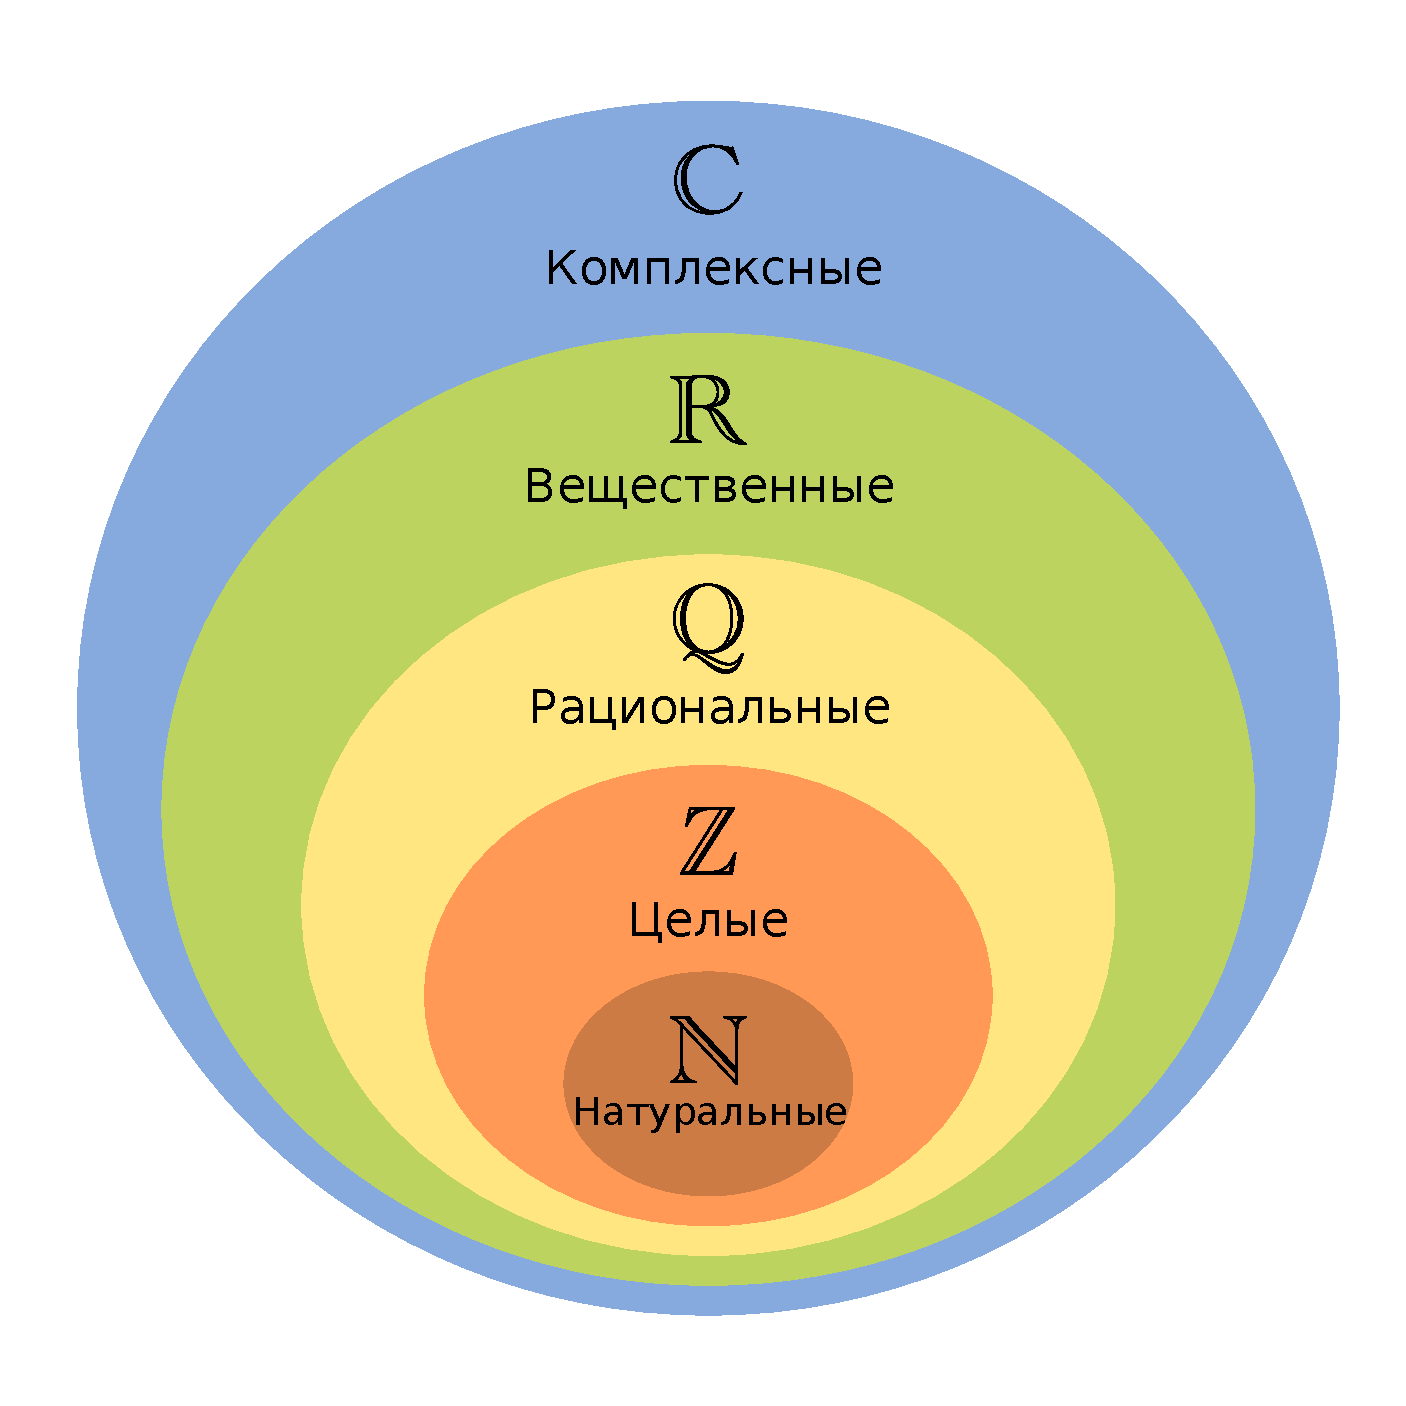
\includegraphics[width=0.5\textwidth]{numbers-types.pdf}
	\caption{Иерархия типов чисел \cite{Wiki:numbers-types}}\label{fig:numbers-types}
\end{figure}

\subsection{Элементарные формулы, уравнения и~пропорции}
\subsubsection{Пропорции}

Две~величины \emph{прямо пропорциональны} друг другу, если изменение значения одной из~них в~$m$~раз влечёт за~собой такое~же изменение другой.
\begin{equation}\label{simple-dir-prop1}
	\begin{aligned}
		\frac{a}{b}=\frac{c}{x} \\
		xa = bc \\
		x = \frac{bc}{a}
	\end{aligned}
\end{equation} 

Две~величины \emph{обратно пропорциональны} друг другу, если увеличение~(уменьшение) значения одной из~них в~$m$~раз влечёт за~собой уменьшение~(увеличение) значения другой также в~$m$~раз.
\begin{equation}\label{simple-inv-prop1}
\begin{aligned}
\frac{a}{b}=\frac{c}{x} \\
xb = ac \\
x = \frac{ac}{b}
\end{aligned}
\end{equation}

\begin{Thexmpl}\label{ex:dir-prop}
	Для~отопления здания строительным объёмом 2000~куб.\,м необходима отопительная система мощностью 68~кВт. Какова потребная мощность отопительной системы для~здания строительным объёмом 2000~куб.\,м?
	
	\begin{equation*}\label{ex:-inv-prop}
	\begin{aligned}
	\frac{68}{2000}=\frac{x}{2500} \\
	2000x = 68\times 2500 \\
	2000x = 170000 \\
	x = \frac{170000}{2000} \\
	x = 85
	\end{aligned}
	\end{equation*}
	
	Ответ: для здания строительным объёмом 2500~куб.\,м необходима система мощностью 85\,кВт.
\end{Thexmpl}

\begin{Thexmpl}\label{ex:inv-prop}
Резец токарного станка утрачивает свои свойства и~нуждается в~обслуживании после 30~дней эксплуатации при~ежедневном односменном использовании (1~смена "--- 8 часов). Через сколько дней потребуется обслуживание резца при~трёхсменной работе?

\begin{equation*}\label{}
\begin{aligned}
\frac{1}{3}=\frac{30}{x} \\
3x = 30 \\
x = \frac{30}{3} \\
x = 10
\end{aligned}
\end{equation*}

Ответ: при~трёхсменной работе обслуживание резца потребуется через 10~дней.
\end{Thexmpl}

\subsubsection{Трансформация бесконечной периодической десятичной дроби в~обыкновенную}

В~ряде случаев возникает потребность трансформации бесконечной периодической десятичной дроби в~обыкновенную. Для~выполнения этой операции следует использовать формулу
\begin{equation}\label{eq:periodic-to-frac-1}
a.b(c)=a\frac{<b><c>-<b>}{x[9]y[0]},
\end{equation}
где $a$ "--- целая часть десятичной дроби,

$b$ "--- не повторяющая часть десятичной дроби,

$c$ "--- периодическая часть десятичной дроби,

$x$ "--- количество цифр 9 в~знаменателе, зависит от~количества чисел в~периодической части $c$,

$x$ "--- количество цифр 0 в~знаменателе, зависит от~количества чисел в~не повторяющейся части $b$.

В~случае отсутствия не~повторяющейся части используется формула
\begin{equation}\label{eq:periodic-to-frac-2}
a.(c)=a\frac{c}{x[9]}
\end{equation}

\begin{Thexmpl}\label{ex:periodic-to-frac-2}
	Вычислим
	$\begin{aligned}
		2.12(3) = 2\frac{123-12}{900} = 2\frac{111}{900} = 2\frac{37}{300} \\
		2.(3) = 2\frac{3}{9} =2\frac{1}{3} 
	\end{aligned}$
	
\end{Thexmpl}

\subsubsection{Работа с~многоэтажными дробями}

С~учётом повсеместного распространения компьютерных вычислений, нет~никакой сложности вычисления многоэтажных дробей. Однако при~работе с~аналитическими методами часто возникает необходимость приведения выражения к~табличному~(стандартному кем-то~уже исследованному) виду. Например, такая потребность возникает при~вычислении производных, дифференциалов и~интегралов, многие из~которых имеют стандартные решения. Умение видеть в~существующем выражении другое, имеющее стандартное решение, и~преобразовать первое ко~второму позволяет экономить много времени. Таким образом, хотя типичный оценщик возможно никогда не~будет вычислять дифференциалы, оценщику, занимающемуся разработкой экспертных систем, подобное знание не~будет лишним.
В~общем виде работа с~многоэтажными дробями выглядит следующим образом
\begin{equation}\label{eq:multilevel-frac}
\frac{\frac{a}{b}}{\frac{c}{d}} = \frac{a}{b} \div \frac{c}{d} = \frac{a}{b} \times \frac{d}{c}
\end{equation}

\subsubsection{Свойства числовых неравенств}
\textbf{Первым свойством неравенств} является сохранение знака неравенства при~сложении его~обеих частей с~константой.
\begin{equation}\label{eq:enequalities-property1}
	\begin{aligned}
	a&>b \\
	a+k&>b+k:\ \forall k\\
	\end{aligned}
\end{equation}

\textbf{Вторым свойством неравенств} является сохранение знака неравенства при~умножении либо делении его~обеих частей на~положительную константу.
\begin{equation}\label{eq:enequalities-property2}
\begin{aligned}
a&>b \\
ak&>bk:\ k>0\\
\end{aligned}
\end{equation}

\textbf{Третьим свойством неравенств} является изменение знака неравенства на~противоположный при~умножении либо делении его~обеих частей на~отрицательную константу.
\begin{equation}\label{eq:enequalities-property3}
\begin{aligned}
a&>b \\
ak&<bk:\ k<0\\
\end{aligned}
\end{equation}

\textbf{Четвёртым свойством неравенств} является возможность почленного сложения неравенств, имеющих одинаковый знак. При~этом знак неравенств сохраняется.
\begin{equation}\label{eq:enequalities-property4}
\begin{aligned}
a>b \\
c>d \\
a+c>b+d\\
\end{aligned}
\end{equation}

\textbf{Пятым свойством неравенств} является возможность почленного вычитания неравенств, имеющих одинаковый знак. При~этом сохраняется знак первого неравенства.
\begin{equation}\label{eq:enequalities-property5}
\begin{aligned}
a>b \\
c<d \\
a-c>b-d\\
\end{aligned}
\end{equation}

\textbf{Шестым свойством неравенств} является возможность их~почленного умножения при~одинаковом знаке с~его~сохранением в~том~случае, когда все~члены неравенств являются положительными числами.
\begin{equation}\label{eq:enequalities-property6}
\begin{aligned}
a&>b \\
c&>d \\
ac&>bd:\ a,b,c,d>0
\end{aligned}
\end{equation}
\textbf{Седьмое свойство неравенств} заключается в~сохранении знака неравенства при~сложении его~членов с~одной и~той~же константой.
\begin{equation}\label{eq:enequalities-property7}
\begin{aligned}
a&>b \\
b&>c \Rightarrow \\
a&>c\\
\end{aligned}
\end{equation}

\textbf{Восьмое свойство неравенств} заключается в~сохранении знака неравенства при~возведении его~членов в~степень с~одинаковым показателем, при~условии положительного значения членов.
\begin{equation}\label{eq:enequalities-property8}
\begin{aligned}
a&>b \Rightarrow\\
a^n&>b^n:\ a,b>0\\
\end{aligned}
\end{equation}

\subsubsection{Системы уравнений с~двумя переменными}

В~общем виде такие уравнения задаются выражением
\begin{equation}\label{eq:systems-linear-equations}
\begin{aligned}
\begin{cases}
a_{1}x+b_{1}y+c_{1}=0\\
a_{2}x+b_{2}y+c_{2}=0
\end{cases}
\end{aligned}
\end{equation}
Решением системы таких уравнений является нахождение \textit{x} и~\textit{y}, удовлетворяющих каждому из~условий. 
\begin{description}
	\item[Корень уравнения] "--- такое значение переменной, при~подстановке которого уравнение обращается в~верное числовое равенство. \textbf{Корень уравнения} с~одной переменной также называют решением уравнения.
\end{description}

Существует несколько методов решения уравнений с~двумя переменными. В~данном материале будут рассмотрены \emph{метод подстановки} и~\emph{метод сложения}. В~первом случае одна из~неизвестных выражается через другую.
\begin{Thexmpl}\label{ex:sys1}
	Дано:
	
	$\begin{aligned}
		\begin{cases}
			2x-y=2 \\
			4x+3y = 9\\
		\end{cases}\\
		\text{Выразим y через x из первого уравнения}\\
		y=2x-2 \Rightarrow 4x+3(2x-2) = 9 \\
		4x+6x-6 = 9 \\
		10x = 15 \\
		x = 1.5 \Rightarrow 3-y=2 \\
		y = 1 \\
		\text{Ответ: x = 1.5, y = 1} \\
		\end{aligned}$
	\end{Thexmpl}
Во~втором случае на~первом этапе одно из~уравнений умножается на~константу так, чтобы при~почленном сложении на~втором этапе одно из~неизвестных уничтожилось. Умножение обоих уравнений на~константы также допускается. При~этом константой может быть любое положительное число.
\begin{Thexmpl}\label{ex:sys2}
	Дано:
	
	$\begin{aligned}
	\begin{cases}
	2x-y=2 \\
	4x+3y=9\\
	\end{cases}\\
	\begin{cases}
	2x-y=2 | \times3 \\
	4x+3y=9\\
	\end{cases}\\
	\begin{cases}
	6x-3y=6\\
	+\\
	4x+3y=9\\
	\end{cases}\\
	10x=15\\
	x=1.5\\
	3y=9-6\\
	y=1\\
	\text{Ответ: x = 1.5, y = 1} \\
	\end{aligned}$
\end{Thexmpl}

\subsubsection{Уравнения с~двумя неизвестными}\label{Two-unknown-1}
В~общем виде уравнение с~двумя неизвестными может быть записано следующим образом.
\begin{equation}\label{eq:two-unknown}
ax+by+c=0:\ a \vee b \neq 0
\end{equation}
Подобные уравнения имеют бесконечное число решений, которые могут быть представлены графически.

\begin{Thexmpl}\label{ex:two-unknown}
	Дано:
	
	$\begin{aligned}
	4x-2y+2=0
	\end{aligned}$
	
	\text{Методом подстановки можно догадаться, что~решением является} x=1, y=3.
	
	\text{Однако решениями будут и~} x=0, y=1, x=-3, y=-2. \text{и~т.\,д.}
		
    \text{Графическое решение показано на~рисунке~\ref{fig:two-unknown}.} 
\end{Thexmpl}

\begin{figure}[ht]
	\centering % Центрируем картинку
	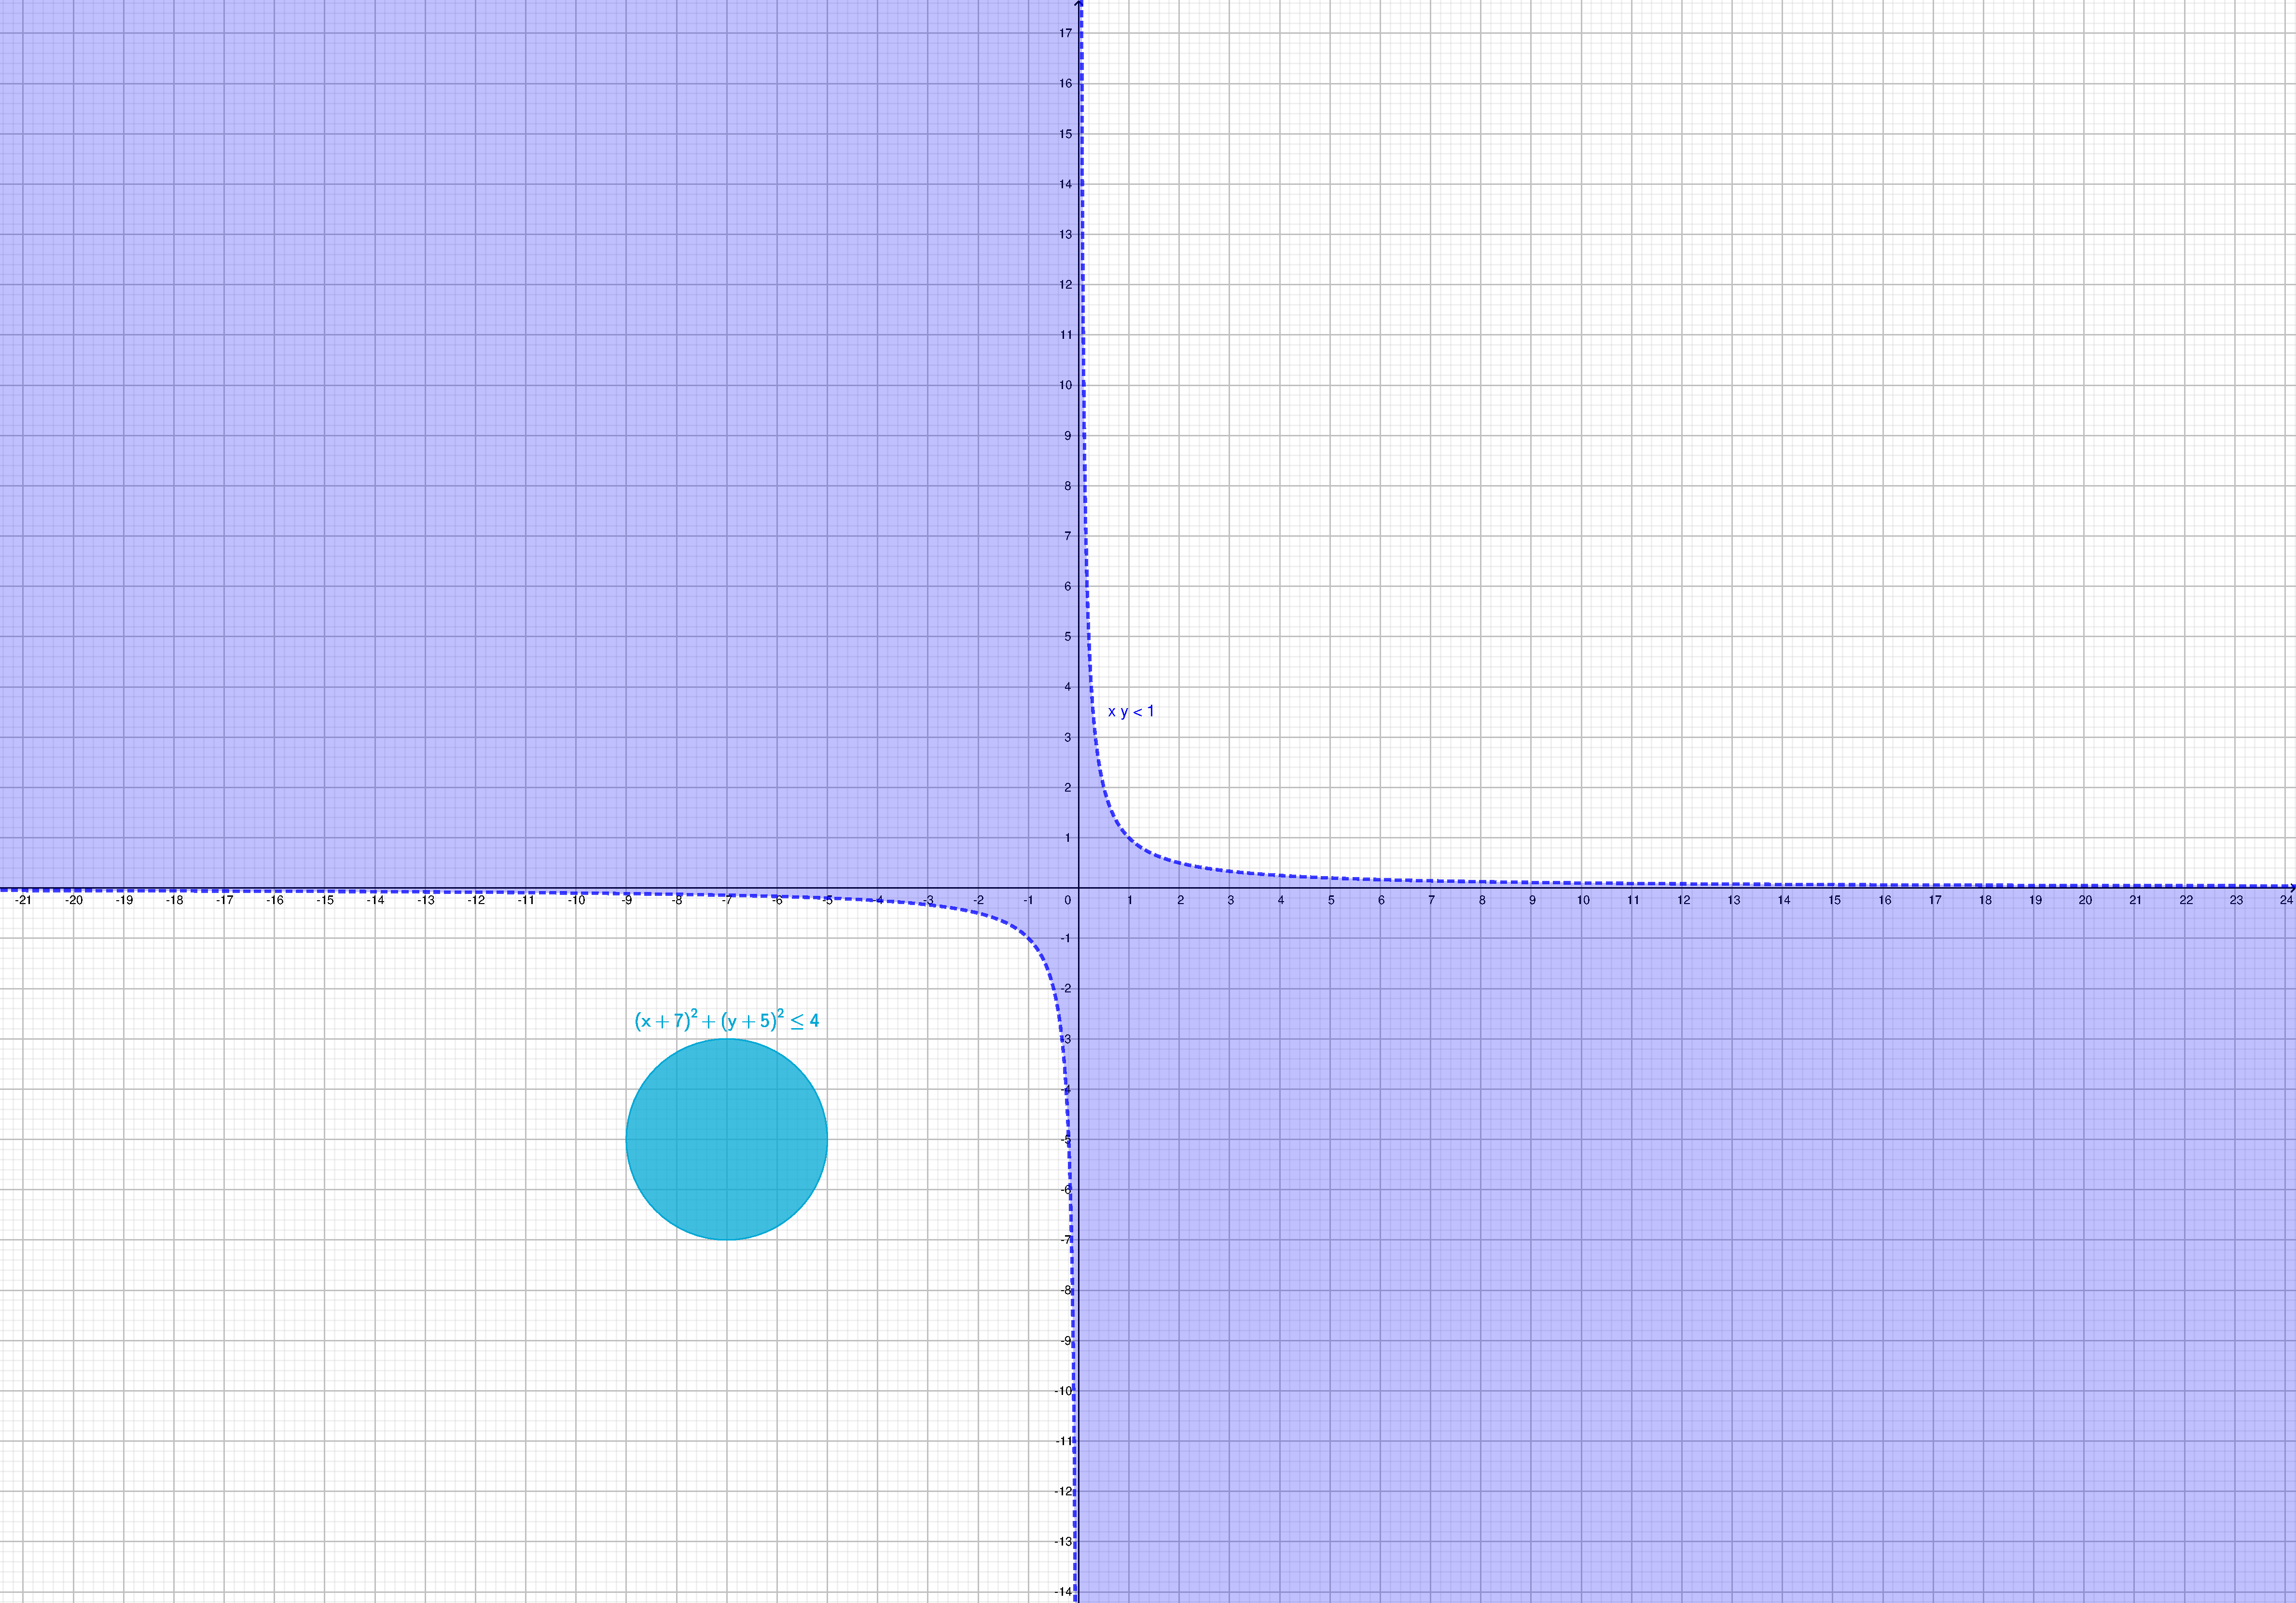
\includegraphics[width=0.5\textwidth]{two-unknown.pdf}
	\caption{Графическое решение уравнения с~двумя неизвестными}\label{fig:two-unknown}
\end{figure}

\subsubsection{Операции со~степенями с~натуральными и~нулевым показателями}

Свойствами степени с~натуральным показателем являются:
\begin{equation}\label{eq:nat-degrees-prop-1}
	\begin{aligned}
	a^n*a^m &= a^{n+m} \\
	\frac{a^n}{a^m} &=a^{n-m} \\
	a^{n^{m}} &= a^{nm} \\
	a^n \times b^n &= (ab)^n \\
	\frac{a^n}{b^n} &= \frac({a}{b})^n \\
	a^0 &= 1: a \neq 0 \\
	0^0 &= \neq \ \exists.
	\end{aligned}
\end{equation}

\subsubsection{Понятие одночлена и~операции с~ним}
\begin{description}
	\item[Одночлен] "--- произведение переменных либо чисел, возведённое в~степень с~натуральным показателем.
\end{description}
Для~работы с~одночленами, как~правило, их~приводят в~стандартный вид, при~котором числовая часть выносится вперёд.
\begin{Thexmpl}\label{ex:monomial-1}
	Дано:
	
	$4x^{3}y^{3}z^{2} \times -2x^{2}y^{2}z^{-1}$
	
	Необходимо привести данный одночлен к~стандартному виду.
	
	Ответ: $-8x^{5}y^{5}z$
\end{Thexmpl}

\begin{description}
	\item[Подобные одночлены] "--- одночлены, состоящие из~одних и~тех~же переменных, возведённых в~степень с~одним и~тем~же показателем.
\end{description}

\subsubsection{Понятие многочлена и~операции с~ним}
\begin{description}
	\item[Многочлен] "--- сумма одночленов.
\end{description}
Для~осуществления операций c~многочленами, как~правило, необходимо привести каждый из~входящих в~него одночленов в~стандартный вид, а~затем привести подобные слагаемые.

Существует ряд стандартных формул для~упрощённого умножения многочленов.

Квадрат суммы двух выражений:
\begin{equation}\label{eq:simple-multipl-of-polynomials-1}
(a+b)^2=a^2+2ab+b^2.
\end{equation}
Квадрат разности двух выражений:
\begin{equation}\label{eq:simple-multipl-of-polynomials-2}
(a-b)^2=a^2-2ab+b^2.
\end{equation}
Разность квадратов двух выражений:
\begin{equation}\label{eq:simple-multipl-of-polynomials-3}
a^2-b^2 = (a-b)(a+b).
\end{equation}
Куб суммы двух выражений:
\begin{equation}\label{eq:simple-multipl-of-polynomials-4}
(a+b)^3 = a^3 + 3a^{2}b+3ab^{2}+b^3.
\end{equation}
Куб разности двух выражений:
\begin{equation}\label{eq:simple-multipl-of-polynomials-5}
(a-b)^3 = a^3 - 3a^{2}b+3ab^{2}-b^3.
\end{equation}
Сумма кубов двух выражений:
\begin{equation}\label{eq:simple-multipl-of-polynomials-6}
a^3+b^3=(a+b)(a^2-ab+b^2),
\end{equation}
где $(a^2-ab+b^2)$ "--- неполный квадрат разности выражений.
Разность кубов двух выражений:
\begin{equation}\label{eq:simple-multipl-of-polynomials-7}
a^3-b^3=(a-b)(a^2+ab+b^2),
\end{equation}
где $(a^2-ab+b^2)$ "--- неполный квадрат суммы выражений.

Применение стандартных формул упрощает работу с~аналитическими выражениями.

\begin{Thexmpl}\label{ex:full-square}
	Земельный участок какой максимальной площади можно огородить, имея ограждение общей длиной 240\,м? Какова длина сторон такого участка, если участок имеет прямоугольную форму? 
	
	Примем длину одной стороны за $x$, тогда другая сторона равна $120-x$.
	
	$S=(120-x)(x)=120x-x^2=-(x^2-30x)$
	
	Выделим полный квадрат выражения.
	
	$-(\underbrace{x^2-2x60+60^2}_{\text{полный квадрат}}-60^2)=3600-(x-60)^2$
	
	Проанализируем полученное выражение. Логично, что~площадь будет максимальной~(3600~кв.\,м) в~том случае, если выражение в~скобке будет равно нулю, что~достигается при~$x=60$. Таким образом, максимально возможная площадь составляет 3600~кв.\,м при~всех сторонах равных 60~м, т.\,е.~тогда, когда участок будет иметь форму квадрата, что~соответствует априорным знаниям.
\end{Thexmpl}

\begin{description}
	\item[Разложение многочлена на~множители] "--- представление многочлена в~виде произведения других многочленов.
\end{description}

\subsubsection{Тождество}
\begin{description}
	\item[Тождество] "--- равенство, являющееся верным при~всех допустимых значения переменных.
\end{description}

Примерами тождеств являются формулы сокращённого умножения~(\ref{eq:simple-multipl-of-polynomials-1}--\ref{eq:simple-multipl-of-polynomials-7}).

\subsubsection{Алгебраические дроби}
\begin{description}
	\item[Алгебраической дробью] называется выражение вида
	\begin{equation}\label{eq:alg-frac}
	\frac{P}{Q}:\ Q \neq 0.
	\end{equation} 
\end{description}
Примерами алгебраических дробей являются, например выражения $\frac{x^2+y}{x}, \frac{x+2}{x-2}, \frac{5}{11}$ и~т.\,д.

\textbf{Основным свойством} \emph{алгебраических дробей} является то, что~при~умножении их~числителя и~знаменателя на~один и~тот~же многочлен, значение алгебраической дроби не~меняется при~условии ненулевого значения такого многочлена.

Из~этого свойства следует возможность сокращения числителя и~знаменателя на~общий множитель.

Для~сложения и~вычитания алгебраических дробей их~следует привести к~общему знаменателю по~обычным правилам.

\begin{Thexmpl}\label{ex:alg-frac-1}
	
	$\begin{aligned}
		\frac{x}{x+y}+\frac{y}{x-y}=\frac{x(x-y)}{(x+y)(x-y)}+\frac{y(x+y)}{(x+y)(x-y)}=\frac{x(x-y)+y(x+y)}{(x+y)(x-y)}=\\
		=\frac{x^{2}-xy+xy+y^{2}}{x^{2}-y^{2}}=\frac{x^{2}+y^{2}}{x^{2}-y^{2}}
	\end{aligned}$
\end{Thexmpl}
Умножение и~деление алгебраических дробей осуществляется согласно общим правилам осуществления таких операций с~дробями.
\begin{equation}\label{eq:alg-frac-multiple}
\frac{a}{b}\times\frac{c}{d}=\frac{ac}{bd}
\end{equation}
\begin{equation}\label{eq:alg-frac-division}
\frac{a}{b}\div\frac{c}{d}=\frac{ad}{bc}
\end{equation}
Возведение алгебраической дроби в~степень осуществляется отдельно для~числителя и~знаменателя.
\begin{equation}\label{eq:alg-frac-power}
(\frac{a}{b})^n=\frac{a^n}{b^n}
\end{equation}

\subsubsection{Рациональные уравнения}
\begin{description}
	\item[Рациональные уравнения] "--- это~выражения вида
	\begin{equation}\label{eq:rational-equations}
	p(x)=0
	\end{equation}
\end{description}

\subsubsection{Степень с~целым отрицательным показателем}
Вычисление степени с~целым отрицательным показателем осуществляется по~формуле
\begin{equation}\label{eq:neg-power}
a^{-n}=\frac{1}{a^{n}}
\end{equation}

\subsubsection{Функция $\sqrt{x}$, её~свойства и~график}
По~свойству квадрата областью определения данной функции являются все~неотрицательные числа, т.\,е. Областью её~значений также являются все~неотрицательные числа.
\begin{equation}\label{eq:sqrt-function-domain}
y=\sqrt{x}
D(y)=[0,+\infty)
E(y)=[0,+\infty)
\end{equation}
Данная функция является возрастающей, т.\,е.~большему значению аргумента соответствует большее значение функции.
$\begin{aligned}
x_2>x_1\\
y_2>y_1\\
\end{aligned}$
График функции $\sqrt{x}$ показан на~рисунке~\ref{fig:sqrt-func}.
\begin{figure}[ht]
	\centering % Центрируем картинку
	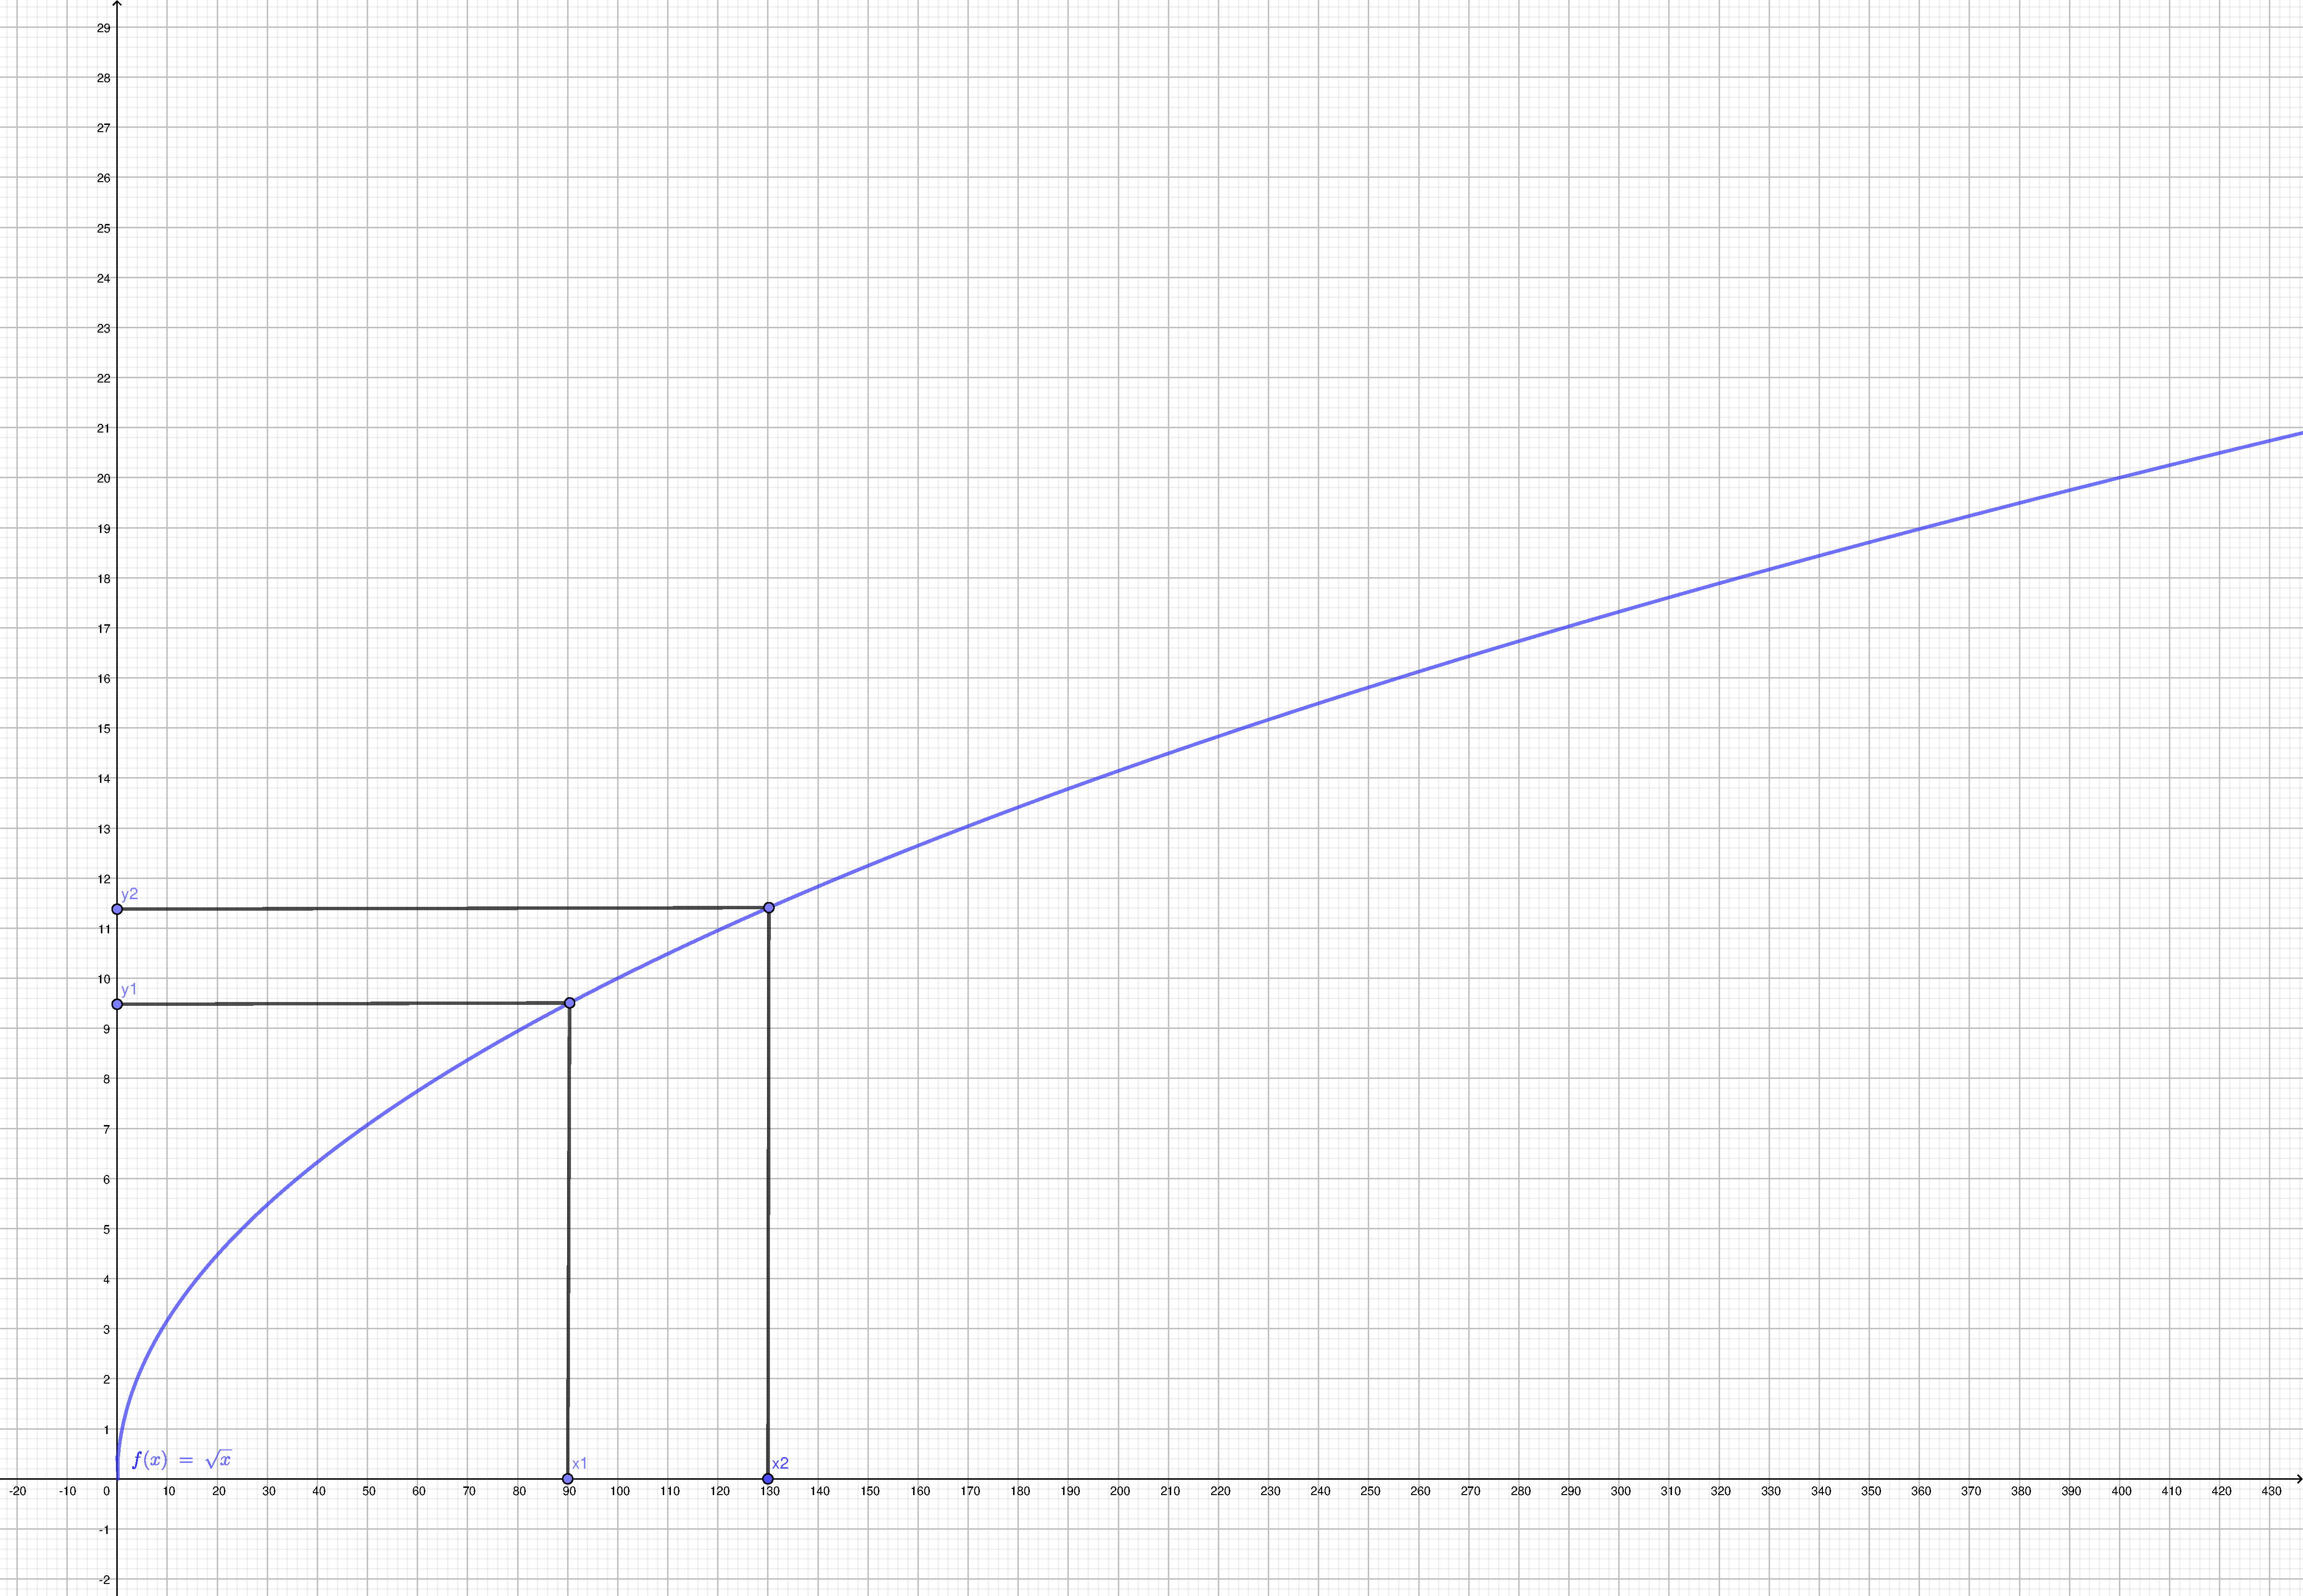
\includegraphics[width=0.8\textwidth]{sqrt-func.pdf}
	\caption{Функция $\sqrt{x}$}\label{fig:sqrt-func}
\end{figure}

\subsubsection{Свойства квадратного корня и~выражения с~ним}
Первое свойство квадратного корня:
\begin{equation}\label{sqrt-prop-1}
\sqrt{ab}=\sqrt{a} \times \sqrt{b}:\ a,b \geq 0.
\end{equation}
Из~этого также следует что
\begin{equation}\label{sqrt-prop-2}
\sqrt{\frac{a}{b}}=\frac{\sqrt{a}}{\sqrt{b}}:\ a,b \geq 0.
\end{equation}
\subsection{Основы геометрии}
\subsubsection{Треугольники и~их~свойства}
\paragraph{Признаки равенства треугольников}
Первым признаком равенства треугольников является признак по~двум сторонам и~углу между ними.
\begin{theorem}
	Если две стороны и~угол между ними одного треугольника соответственно равны двум сторонам и~углу между ними другого треугольника, то~эти~треугольники равны.
\end{theorem}
Вторым признаком равенства треугольников является признак по~двум углам и~стороне между ними.
\begin{theorem}
	Если сторона и~два~прилежащих угла одного треугольника соответственно равны стороне и~двум прилежащим углам другого треугольника, то~эти~треугольники равны.
\end{theorem}
Вторым признаком равенства треугольников является признак по~трём сторонам.
\begin{theorem}
	Если все~стороны треугольника соответственно равны сторонам другого треугольника, то~эти~треугольники равны.
\end{theorem}

\paragraph{Замечательные прямые и~точки треугольника}
В~данном материале будут рассмотрены простейшие замечательные прямые:
\begin{itemize}
	\item медиана;
	\item биссектриса;
	\item высота;
	\item прямая Эйлера,
\end{itemize}
а~также простейшие замечательные точки:
\begin{itemize}
	\item центроид;
	\item инцентр;
	\item ортоцентр.
\end{itemize}

\begin{description}
	\item[Медиана треугольника] "--- отрезок, соединяющий вершину треугольника с~серединой противоположной стороны. Иногда \emph{медиано}й называют также прямую, содержащую этот отрезок. Точка пересечения медианы со~стороной треугольника называется \textbf{основанием медианы}.
\end{description}
Все~три медианы треугольника пересекаются в~одной точке, которая называется \textbf{центроидом} либо центром тяжести треугольника, и~делятся этой точкой на~две части в~отношении 2:1, считая от~вершины.

На~рисунке~\ref{fig:triangle-lines-points} медианы выделены синим цветом, а~центроидом является точка~H.

\begin{description}
	\item[Медиана треугольника] "--- отрезок, соединяющий вершину треугольника с~серединой противоположной стороны. Иногда \emph{медиано}й называют также прямую, содержащую этот отрезок. Точка пересечения медианы со~стороной треугольника называется \textbf{основанием медианы}.
\end{description}
Все~три медианы треугольника пересекаются в~одной точке, которая называется \textbf{центроидом} либо центром тяжести треугольника, и~делятся этой точкой на~две части в~отношении 2:1, считая от~вершины.

На~рисунке~\ref{fig:triangle-lines-points} \emph{медианы треугольника} выделены синим цветом, а~точка~H является его~\emph{центроидом}.

\begin{description}
	\item[Биссектриса треугольника] "--- отрезок биссектрисы угла, проведённый от~вершины угла до~её~пересечения с~противолежащей стороной. Точка пересечения биссектрисы угла треугольника с~его стороной, не~являющейся стороной этого угла, называется \textbf{основанием биссектрисы}.
\end{description}

Все~три биссектрисы внутренних углов треугольника пересекаются в~одной точке, называемом \textbf{инцентр} и~являющейся центром вписанной в~этот треугольник окружности.

На~рисунке~\ref{fig:triangle-lines-points} \emph{биссектрисы} выделены зелёным цветом, а~точка~J является \emph{инцентром}.

\begin{description}
	\item[Высота треугольника] "--- перпендикуляр, опущенный из~вершины треугольника на~противоположную сторону (точнее, на~прямую, содержащую противоположную сторону).
\end{description}
В зависимости от типа треугольника высота может содержаться внутри треугольника (для остроугольного треугольника), совпадать с его стороной (являться катетом прямоугольного треугольника) или проходить вне треугольника у тупоугольного треугольника. Все 3 высоты треугольника пересекаются в~1 точке, называемой \textbf{ортоцентром}.

На~рисунке~\ref{fig:triangle-lines-points} \emph{высоты}~(и~их~продолжения) выделены фиолетовым цветом, а~точка~M является \emph{ортоцентром}.

\begin{description}
	\item[Пряма́я Э́йлера] "--- прямая, проходящая через центр описанной окружности и ортоцентр треугольника.
\end{description}

На~рисунке~\ref{fig:triangle-lines-points} \emph{прямая Эйлера}  выделена оранжевым цветом.

\begin{figure}[ht]
	\centering % Центрируем картинку
	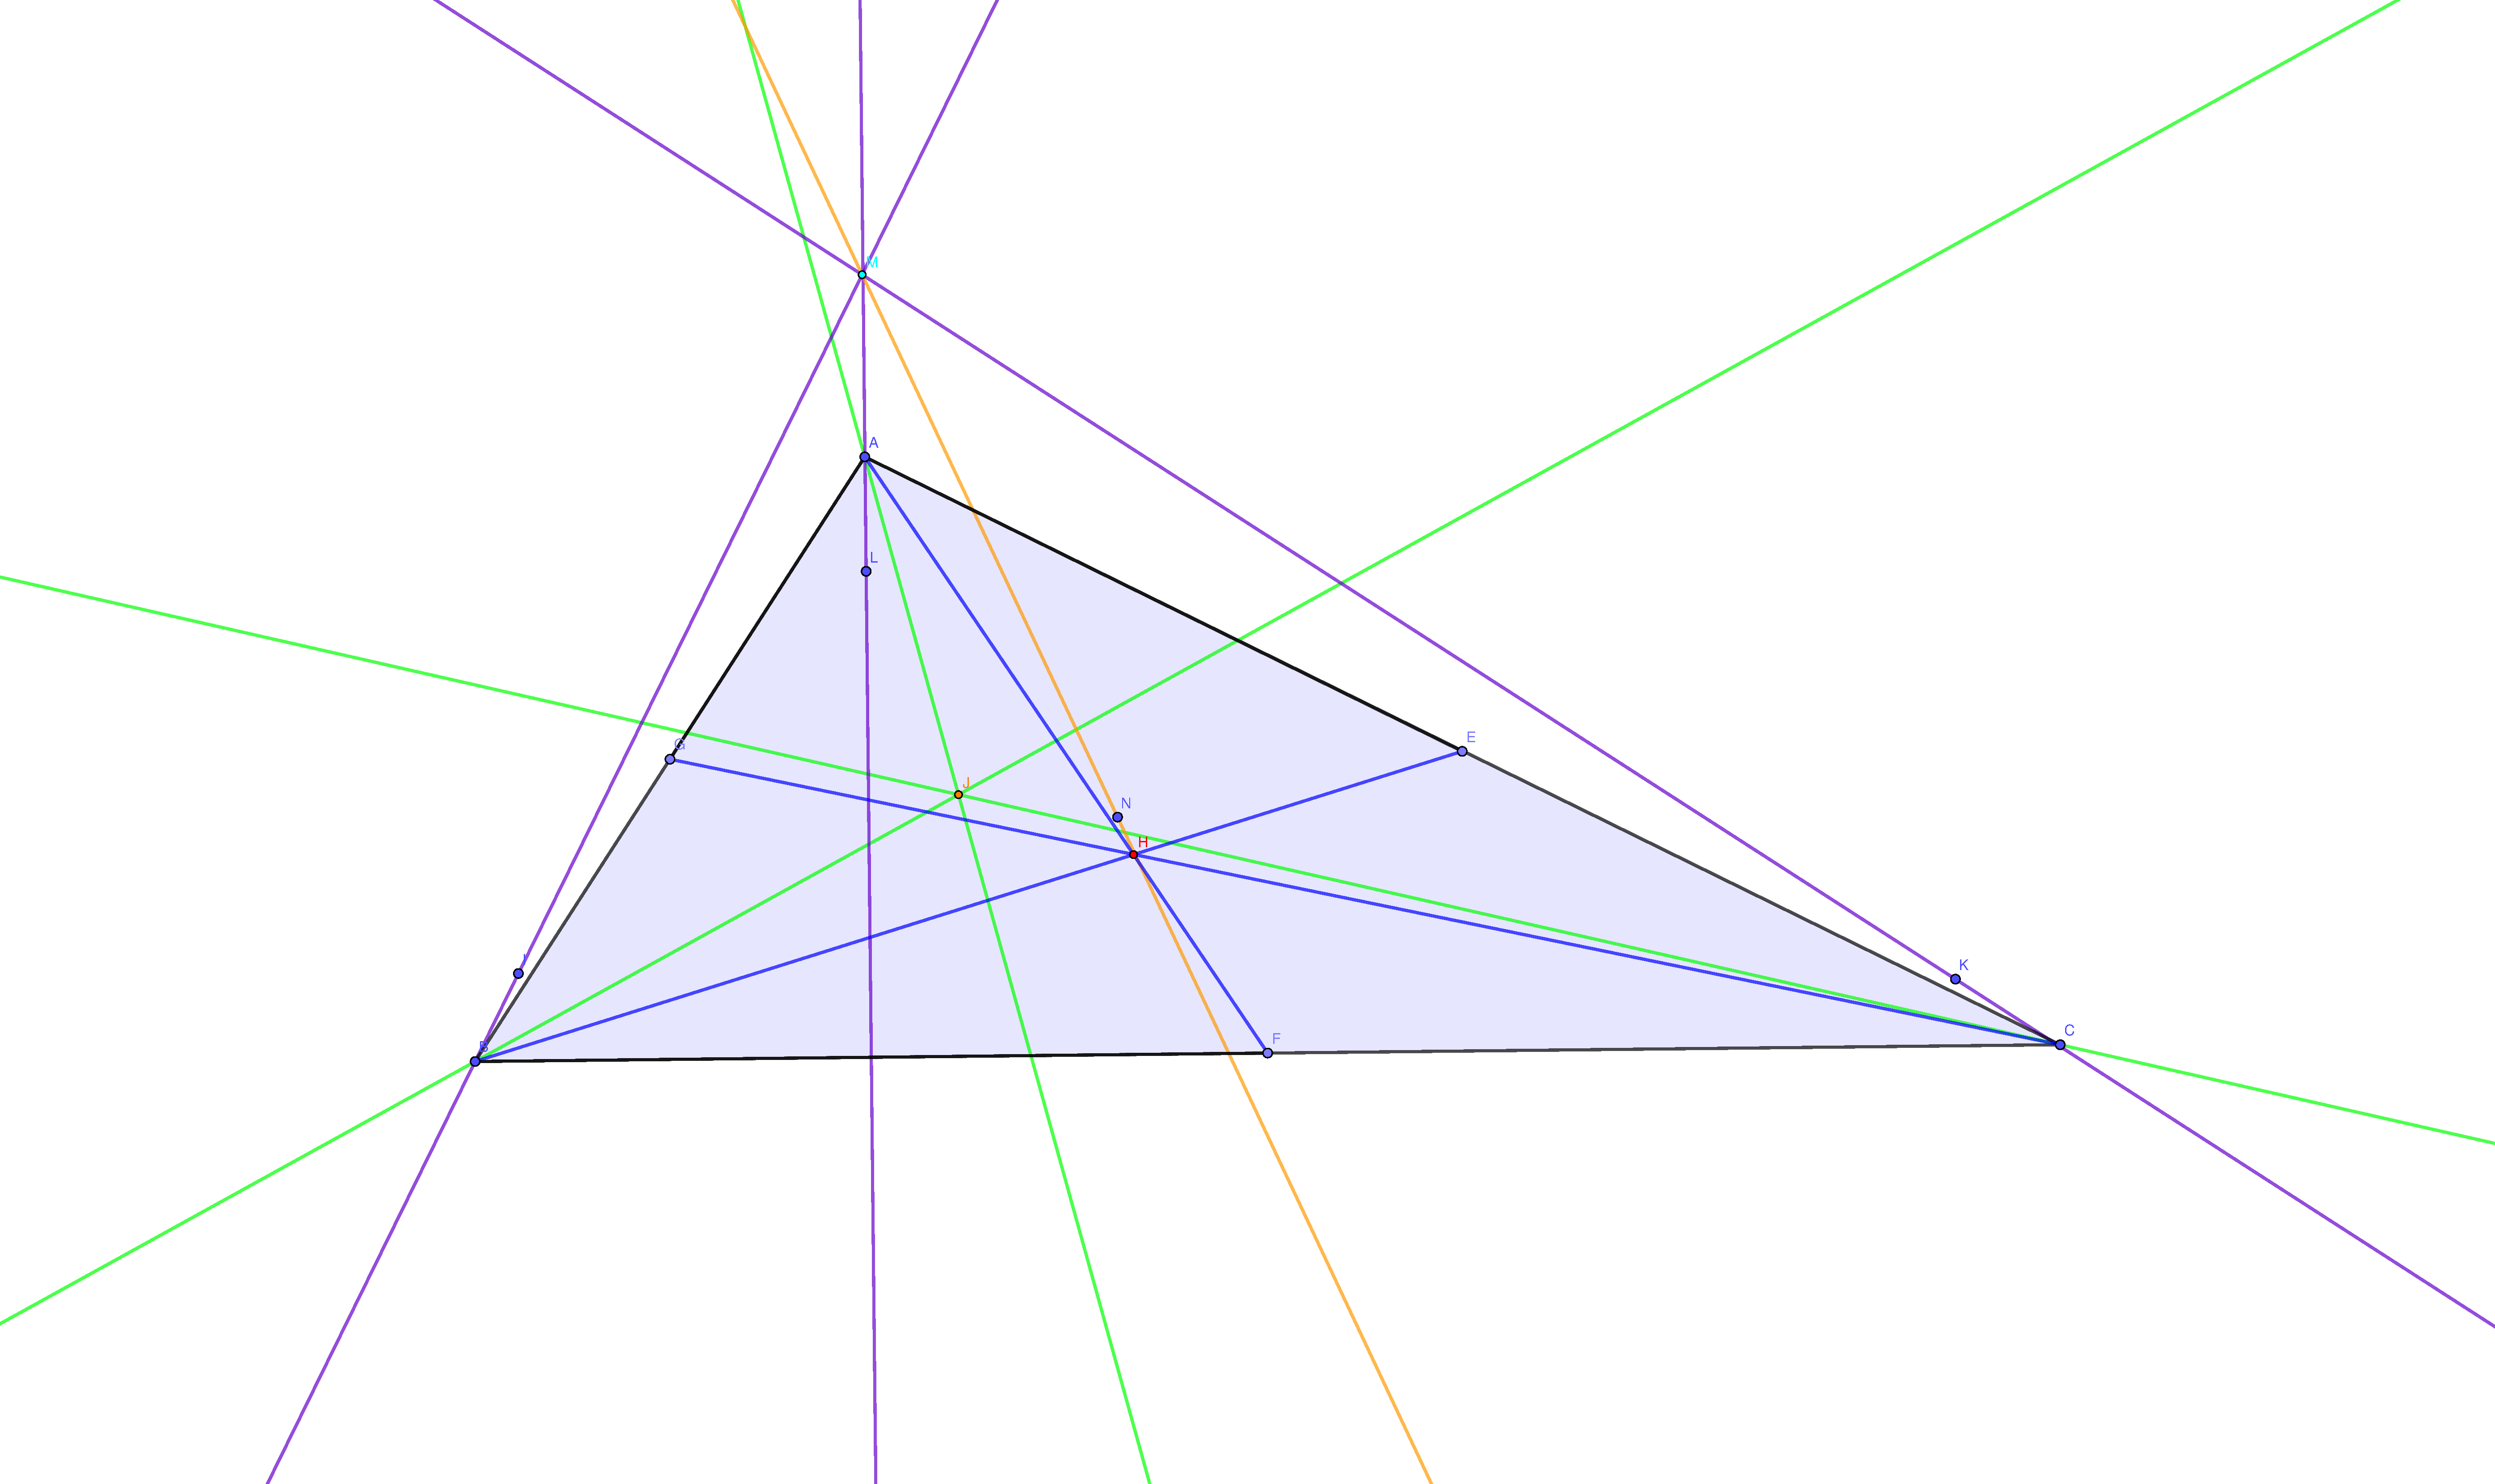
\includegraphics[width=0.8\textwidth]{triangle-lines-points.pdf}
	\caption{Основные замечательные прямые и~точки треугольника}\label{fig:triangle-lines-points}
\end{figure} 


\subsection{Функции}
\subsubsection{Понятие функции}
\textbf{Функция} является одним из~самых важных понятий в~математике.
\begin{description}
	\item[Функция] "--- инструкция (набор инструкций) в~соответствии с~которой каждому элементу первого множества соответствует один и~только один элемент второго множества.
\end{description}
В~общем виде функцию можно записать следующим образом.
\begin{equation}\label{function}
y=f(x),
\end{equation}
где y "--- зависимая переменная (значение функции),

x "--- независимая переменная (аргумент функции),

f "--- выражение.

Одним из~ключевых понятий являются \textbf{область определения функции} и~\textbf{область значения функци}и.
\begin{description}
	\item[Область определения функции] "--- все~возможные значения независимой переменной, при~которых существуют значения зависимой переменной.
\end{description}
Область определения функции записывается следующим образом.
\begin{equation}\label{eq:function-domain}
D(f)
\end{equation}
\begin{description}
	\item[Область значения функции] "--- все~возможные значения зависимой переменной.
\end{description}
Область значения функции записывается следующим образом.
\begin{equation}\label{eq:function-exists}
E(y)
\end{equation}

\subsubsection{Линейная функция и~её~график, взаимное расположение графиков линейных функций}

Общая формула линейной функции следует из~\ref{eq:two-unknown} и~представляет собой выражение
\begin{equation}\label{eq:linear-func-1}
ax+by+c=0: b\neq 0.
\end{equation}
Отсюда следует
\begin{equation}\label{eq:linear-func-2}
	\begin{aligned}
		by &= -ax-c\\
		y &= -\frac{a}{b}x - \frac{c}{b}\\
		k &= -\frac{a}{b}, m &= -\frac{c}{b} \Rightarrow \\
		y &= kx+m. 
	\end{aligned}
\end{equation}
Последнее выражение $y=kx+m$ называется \emph{линейной функцией}, в~которой $x$ "--- независимая переменная~(аргумент), $y$ "--- зависимая переменная (зачение функции). Графиком линейной функции является прямая.

Для~определения взаимного расположения графиков двух линейных функций
\begin{equation*}\label{eq:linear-func-3}
\begin{aligned}
y&=k_{1}x+m_1\\
y&=k_{2}x+m_2\\
\end{aligned}
\end{equation*}
следует использовать правила: в~случае, когда $k_1=k_2, m_1 \neq m_2$ "--- графики функций параллельны; в~случае, когда $k_1=k_2, m_1=m_2$ "--- графики функций совпадают; в~случае, когда $k_1 \neq k_2, m_1 \neq m_2$ "--- графики функций имеют пересечение, являющееся единственным. 

Для~поиска точки пересечения графиков можно использовать следующую простую логику: если выполняется условие пересечения графиков функций, следовательно существует такая единственная точка, в~которой $y_1=y_2$, следовательно $=k_{1}x+m_1 = k_{2}x+m_2$. Далее путём решения простого линейного уравнения можно найти $x$.

\begin{Thexmpl}\label{ex:two-linear-1}
	Дано:
	
	$\begin{aligned}
	y_{1}&=8x - 3\\
	y_{2}&=3x + 2\\
	\end{aligned}$
	
	Найти точку пересечения этих функций. Поскольку коэффициенты перед $x_1, x_2$ разные, следовательно графики функций имеют пересечение, а~значит существует такая единственная точка~в~которой выполняется условие~$y_1=y_2$. Соответственно в~этой точке $8x - 3 = 3x + 2$. Тогда $5x=5$. Из~этого следует, что~$x=1$. Подставив значение $x$ в~любую из~функций получим $y=5$.
	
	Ответ: графики функций пересекаются в~точке~(1, 5).
\end{Thexmpl}

\section{Последовательности}
\subsection{Понятие множества}\label{multiple:definition}
Под~\emph{множеством} понимают совокупность, класс или~собрание объектов безразлично какой природы. Согласно определению основоположника теории множеств \href{https://ru.wikipedia.org/wiki/Кантор,_Георг}{Г.\,Кантора}~\cite{Wiki:Kantor}, множество "--- это~собрание предметов одинаковых или~различных между собой, мыслимое как единое целое. Собрание предметов рассматривается как~один предмет. Не~следует понимать множество как~совокупность действительно существующих предметов, принадлежность предметов одному множества не~требует от~них~сосуществования во~времени и~пространстве. В~логике множество понимается как~абстрактный объект, в~котором каждый предмет рассматривается с~точки зрения признаков, по~которым данный предмет принадлежит данному множеству. В~множестве предметы становятся неразличимыми друг от~друга по~признакам и~их~только по~именам.

Объект, принадлежащий данному множеству, называется его~\textbf{элементом}. Множество обозначается заглавными латинскими буквами ${\text{A}, \text{B}, \text{C}\ldots}$. Элементы, входящие в~множество, обозначаются строчными латинскими буквами и~заключаются в~фигурные скобки: ${\{a,b,c\}}$.

Множество, содержащее конечное число элементов, называется \textbf{конечным}, а~бесконечное число элементов "--- \textbf{бесконечным}.

Два множества называются \textbf{равными}, если содержат одинаковые элементы ${(\text{A}={2,4,8}=\text{B}={2,2,4,8})}$.

Элементами множества могут быть другие множества ${\text{A}={{2,3},{4,5}}}$. При~этом ${\text{A}={{2,3},{4,5}}\neq \text{B}= {2,3,4,5}}$.

\emph{Множество}, не~содержащее ни~одного элемента, называется \textbf{пустым множеством}.

\emph{Пустое множество} и~само множество~$А$ называются \textbf{несобственными} подмножествами множества~$А$, все~остальные подмножества "--- \textbf{собственными}.

\emph{Множество} называется \textbf{заданным}, если перечислены все~входящие в~него элементы либо определены признаки, по~которым данный объект можно отнести к~данному множеству:
\begin{description}
	\item[$A=\{x, P(x)\}$] "--- $x$ "--- элементы множества, $P(x)$ "--- свойства элементов данного множества.
	\item[$B=\{x, x=2n, n \in \mathbb{N}\}$] "--- множество чётных чисел.
\end{description}

Если \emph{множество} задано своим свойством, то~нельзя заранее сказать, будут~ли в~нём элементы.

Если множество $A$ содержит $n$ элементов, количество его~подмножеств составляет
\begin{equation}\label{n-submultitudes}
|M_{a}| = 2^n,
\end{equation}
где $n$ "--- число элементов множества.

\begin{Thexmpl}
	Дано:
	
	$\text{A}={\{a, b, c, d, e, f ,g\}}$
	
	$\text{B}={\{f, g, v, w, x, y, z\}}$
	
	$\text{C}={\{a, b\}}$
	
	Тогда:
	
	$C \subset A$
	
	$A \bigcup B = {\{a, b, c, d, e, f, g, v, w, x, y, z\}}$
	
	$A \bigcap B = {\{f, g\}}$
	
	$A \backslash B = {\{a, b, c, d, e\}}$
	
	$B \backslash A = {\{v, w, x, y, z\}}$
	
	$A \triangle B = {\{a, b, c, d, e, v, w, x, y, z\}}$
\end{Thexmpl}


\begin{Thexmpl}
	Дано: $\text{A}={{a, b, c}},\ n = 3$
	
	Вычислить число подмножеств $A$.
	
	$2^3 = 8$
	
	$M_A = \{\text{\AE{}}, a, b, c, \{ab\}, \{ac\}, \{bc\}, \{a,b,c\}\}$
	
	$M_A = 8$
\end{Thexmpl}

\begin{theorem}
	Пустое множество является подмножеством любого множества.
\end{theorem}
End.\cite{Studopedia:mnozhestvo}
\subsection{Понятие отображения множеств}
Большую роль в~математике имеет установление связей между двумя множествами $X$ и~$Y$, связанное с~рассмотрением пар объектов, образованных из~элементов первого множества и~соответствующих им~элементов второго множества. Особое значение при~этом имеет \emph{отображение множеств}.

Пусть $X$ и~$Y$ "--- произвольные множества. Отображением множества $X$ на~множество $Y$ называется $\forall$ правило $f$, по~которому каждому элементу множества $X$ сопоставляется вполне определённый~(единственный) элемент множества~$Y$. Тот~факт, что~$f$ есть отображение $X$ в~$Y$, кратко записывают в~виде: $f:X->Y$.

Таким образом, для~того чтобы задать отображение~$f$ множества~$Х$ в~множество $Y$, надо каждому элементу $x\in X$ поставить в~соответствие один и~только один элемент~$y \in Y$. Если при~этом элементу~$х \in Х$ сопоставлен элемент~$y \in Y$, то~$y$ называют \textbf{образом элемента}~$х$, а~$х$ "--- \textbf{прообразом элемента}~у при~отображении~f, что~записывается в~виде $f(x)=y$.

Из определения отображения~$f$ следует, что~у~каждого элемента~$x$ из~$Х$ есть только один \emph{образ} в~$Y$, однако для~элемента $y$ из~$Y$может быть несколько \emph{прообразов}. Множество всех прообразов элемента~$y$ из~$Y$ называется его~\emph{полным прообразом} и~обозначается через $f^{-1}(y)$. Таким образом, $f^{-1}(y)={x \in X | f(x) \in y}$.

Если множества $Х$ и~$Y$ числовые, то~$f$ называется \textbf{функцией}.

На~первый взгляд может показаться, что~всё~вышеизложенное не~имеет отношения к~оценочной деятельности и~не~имеет практического применения в~ней. Однако данное мнение является заблуждением. Оценщики очень часто сталкиваются с~понятием \emph{функции}. Например, замена исходных значений признака на~его квадрат либо логарифм являются типичными примерами отображения множеств. Так, например в~\cite{Laskin:lognorm} утверждается, что~использование логарифмов значений цен позволяет избежать систематического завышения результатов оценки. В~таблицах~\ref{tab:function-square}, \ref{tab:function-log} показаны примеры отображения при~которых $f$ представляет собой операцию возведения числа в~квадрат и~операцию логарифмирования соответственно.

\begin{table}[ht]
	\caption{Отображение множества при $f=^2$} \label{tab:function-square}
	\centering% центрируем таблицу
	\begin{tabular}{ccc} 
		\hline
		x  & f & y 
		\\ \hline \hline
		-5 & $^2$ & 25 \\ 
		-2 & $^2$ & 4 \\ 
		-1 & $^2$ & 1 \\ 
		0 & $^2$ & 0 \\ 
		1 & $^2$ & 1 \\ 
		2 & $^2$ & 4 \\ 
		5 & $^2$ & 25 \\
		\hline	
	\end{tabular}
\end{table}

\begin{table}[ht]
	\caption{Отображение множества при~$f=log$} \label{tab:function-log}
	\centering% центрируем таблицу
	\begin{tabular}{ccc} 
		\hline
		x  & f & y 
		\\ \hline \hline
		1 & log & 0.000 \\ 
		2 & log & 0.693 \\ 
		3 & log & 1.099 \\ 
		5 & log & 1.609 \\ 
		8 & log & 2.079 \\ 
		13 & log & 2.565 \\ 
		21 & log & 3.045 \\ 
		\hline	
	\end{tabular}
\end{table}

\subsection{Примеры последовательностей}
Последовательностью называется отображение множества натуральных числе во~множество вещественных чисел, т.\,е.~$\mathbb{N} -> \mathbb{R}$. Наиболее простым и~очевидным способом задания последовательности явным образом путём перечисления её~членов, например $x_1, x_2, x_3, x_4,\ldots, x_n$. Можно также использовать задание последовательности с~помощью формул либо словесных описаний. Например, последовательность квадратов натуральных чисел можно задать с~помощью формулы
\begin{equation}\label{eq:conseq-squares}
x_n=x^2.
\end{equation}
Последовательность десятичных знаков числа $\pi$ может быть задана формулой
\begin{equation}\label{eq:conseq-pi}
x_n=\frac{[10^{n-1}\pi]}{10^{n-1}}
\end{equation}
В~ряде случаев задание последовательности может быть выполнено графически. Например для~задания последовательности $1, 0, -1, 0, 1, 0, -1, 0, 1,\ldots$ можно использовать функцию
\begin{equation}\label{eq:sinus}
x_n=\sin \frac{\pi n}{2}.
\end{equation}
Графически такое отображение показано на~рисунке~\ref{fig:sinus}, на~котором заглавными латинскими буквами показаны элементы последовательности.
\begin{figure}[ht]
	\centering % Центрируем картинку
	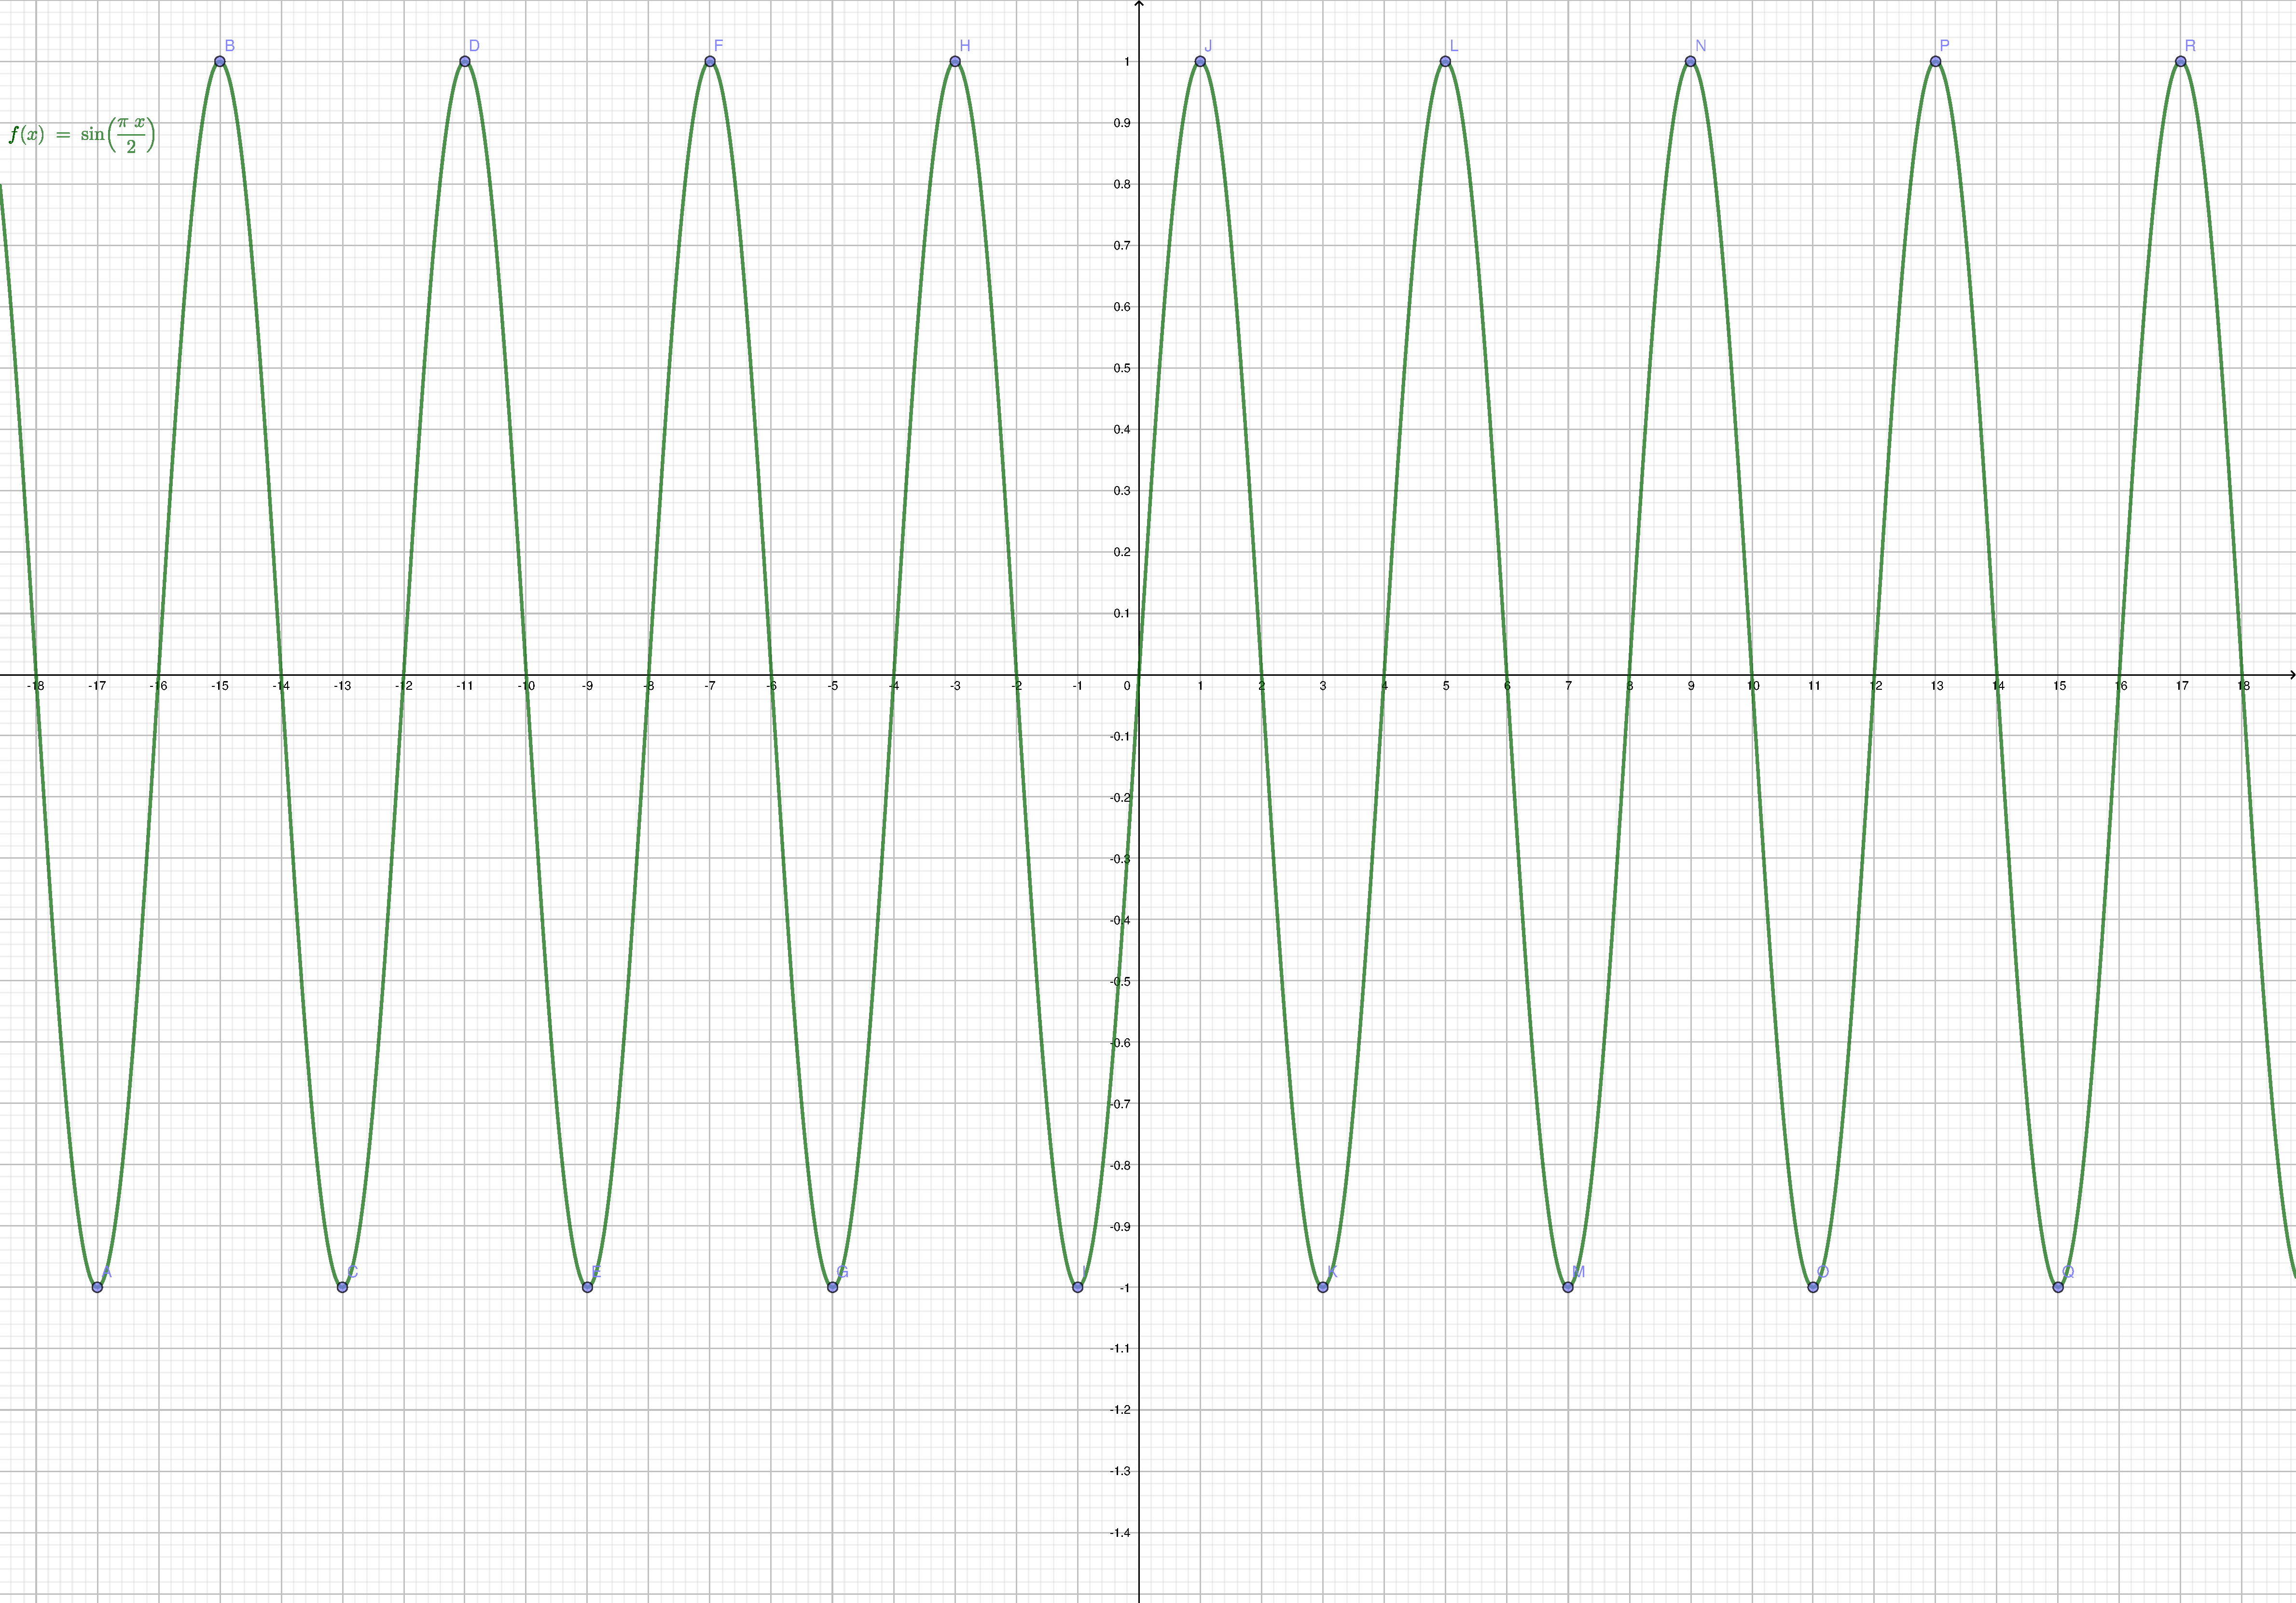
\includegraphics[width=\textwidth]{sinus.pdf}
	\caption{Графическое отображение последовательности $1, 0, -1, 0, 1, 0, -1, 0, 1,\ldots$ )}\label{fig:sinus}
\end{figure}
\subsection{Пределы последовательностей}
Рассмотрим для~примера уже~знакомую ранее последовательность $1, 0, -1, 0, 1, 0, -1, 0, 1,\ldots$, а~затем другую: $1, 1.5, 1,41666, 1.41421566862\ldots, 1.4142135623\ldots$, задаваемую рекуррентно с~помощью формулы
\begin{equation}\label{eq:recurr}
y_{n+1}=\frac{1}{2}(y_n+\frac{2}{y_n}), y_1=1.
\end{equation}
Как~видно, данные последовательности имеют принципиальное отличие: члены первой последовательности чередуются, второй "--- приближаются к~некоторому числу~(квадратному корню из~числа 2).
Предел последовательности имеет форму записи
\begin{equation}\label{eq:limit1}
\lim_{n\to\infty}x_n=l.
\end{equation}
Данную запись можно описать как:
\begin{itemize}
	\item $l$ есть предел последовательности $x_n$ либо
	\item последовательность $x_n$ сходится к~$n$, либо
	\item последовательность $x_n$ стремится к~$n$.
\end{itemize}
Из~этого следует, что~для~любого интервала, содержащего точку $l$, вне~его~находится лишь конечное число последовательности. При~этом неважно, является данный интервал произвольным либо симметричным относительно этой точки, поскольку любой интервал может быть уменьшен либо увеличен для~симметричного. Таким образом во~всех случаях можно вести речь о~симметричных интервалах. Из~этого следует:
\begin{itemize}
	\item при~любом $\epsilon > 0$ вне~интервала $(l-\epsilon, l+\epsilon)$ находится лишь конечное число членов последовательности;
	\item для~любого $\epsilon > 0$ найдётся такой номер $N$, что~$|x_n-l| < \epsilon$, при~всех $n \geq N$;
	\item с~помощью кванторов, описанных в~\ref{mathan-gloss-symbols}, два~вышеуказанных утверждения можно записать кратко: $\forall \epsilon > 0 \quad \exists \quad N \qquad \forall n \geq N \qquad |x_n-l|<\epsilon$.
\end{itemize}
Рассмотрим пример. Возьмём последовательность
\begin{equation}\label{eq:limits2}
\lim_{n\to\infty}\frac{n^2}{n^2+1}=1
\end{equation}
и~покажем, что~она стремится к~$1$. Для~этого оценим модуль разности и~найти такое $n$, при~котором он~будет меньше~1.
\begin{equation}\label{eq:limits3}
|\frac{n^2}{n^2+1}-1|=\frac{1}{n^2+1}<\frac{1}{n^2}<\epsilon \quad \text{при}~n \geq [\epsilon^{(-\frac{1}{2})}+1].
\end{equation}


\section{Логарифмы}
\section{Функции и~непрерывность}
\section{Производные}
\section{Интегралы}




\nocite{CSC:intro-in-matan}

\printbibliography[title=Источники информации]

\end{document}
